 \documentclass[student, noshadow, lsr, english, aspectratio=169]{ITR_LSR_slides}
% student options:
% lsr 				-> lsr, template (remove for itr)
% english 			-> enables english language format
% aspectratio=43	-> 4:3 layout
\usepackage{tikz}
\usepackage{pgfplots}
\pgfdeclarelayer{background}
\pgfdeclarelayer{nodelayer}
\pgfdeclarelayer{edgelayer}
\pgfdeclarelayer{foreground}
\pgfsetlayers{background,edgelayer,nodelayer,main,foreground}
\tikzset{robotRec/.style={rectangle, draw=black,line width=2.5pt, fill=tum_gray, rounded corners=9pt, minimum width=60pt, minimum height=30pt}}
\tikzset{robotCirc/.style={circle, draw=black, fill=black, line width=1.5pt}}
% robot name for tikz figure
\newcommand{\RobotName}{$\mathbf{R}$}
\addbibresource{ref.bib}
\graphicspath{{pics/}{logos/}}

\title{Numerical Discretization in High Accuracy MPC Applications}
\presenter{B.Sc. Tianyuan Kong}

\supervisor{M.Sc. Johannes Teutsch}
\typeofpres{Forschungspraxis}

\usepackage[bigfiles]{media9} %option bigfiles not needed for xelatex, runs without problems on ubuntu14
\usepackage{amsmath}
\usepackage{xcolor}
\usepackage{float}
\usepackage{caption}
\usepackage{subcaption}
\usepackage{amsmath,amssymb,amsfonts}
\usepackage{algorithmic}
\usepackage{graphicx}
\usepackage{textcomp}
\usepackage{diagbox}
\usepackage{mwe} % for blindtext and example-image-a in example
\usepackage{wrapfig}
\usepackage[labelformat=empty]{caption}
\usepackage{graphics}
%%%%%%%%%%%%%%%%%%%%%%%%%%%%%%%%%%%%%%%%%%%%%%%%%%%%%%%%%%%%%%%%%%%%%%%%%%%%%%%%

\begin{document}


\begin{frame}
    \titlepage
\end{frame}


\section{Overview}

\begin{frame}
	\frametitle{Motivation}
	\textbf{MPC on continuous-time systems:}
	\begin{itemize}
		\item[~]
		\item $\text{Continuous-time system} \xrightarrow{\text{numerical} \ \text{discretization}} \text{Discrete-time model} $
		\item[~]
		\item[~]
		\item Zero-order hold control inputs in the discrete-time model
		\item[~]
		\item[~]
		\item Higher accuracy vs. increased computational load
	\end{itemize}
\begin{itemize}
	%\item $\text{Continuous-time system} \xrightarrow{\text{numerical} \ \text{discretization}} \text{Discrete-time model} $
	\item[~]
	%\item Zero-order hold vs. First-order hold Control inputs
\end{itemize}
 %   \\[2ex]
\begin{block}{Goal:}
	\begin{itemize}
		\item Trade-off between prediction accuracy and computational complexity
		\item Zero-order hold vs. Higher-order hold control inputs
	\end{itemize}
\end{block}
\end{frame}

\begin{frame}
	\frametitle{Introduction/Agenda}
    \begin{itemize}
    	\item Runge Kutta (RK) method
    	\item[~]  
    	\item Gauss collocation method
    	\item[~]
    	\item RK: Simulation setup and results
    	\item[~]
    	\item Gauss collocation and FOH: Simulation setup and results
    	\item[~]
    	\item Conclusion
    \end{itemize}
% EPS tutorial
%\begin{figure}[htb]
%\centering
%\psfrag{q1}[Bl][Bl]{\small $\alpha$}
%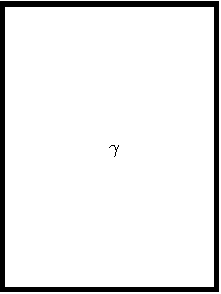
\includegraphics[width=0.9\textwidth]{samplefigure.eps}
%\caption{Sample Figure}
%\end{figure}

\end{frame}

%\begin{frame}
%	\frametitle{Related Work}
%    Normal cite: \cite{buss11}\\
%	Bigger cite: \scite{buss11}\\
%	Multiple  authors: \cite[3]{bauer09}
%\end{frame}

\section{Methods}

\begin{frame}
	\frametitle{Runge Kutta method}
$$
\dot{x} = f(t,x,u) = A_{\rm {con}}x + B_{\rm {con}}u \xrightarrow{\text{RK}\ \text{method}} x_{k+1}= A_{\rm{rk}}x_k + B_{\rm{rk}}u_k
$$
The family of explicit RK methods is given by %\cite{press2007section}
\begin{equation}
	x_{k+1} = x_k +  \sum_{i=1}^s b_i \kappa_i,
\end{equation}
where
\begin{equation}
	\begin{split}
		%\frac{dx}{dt} &=  f(t, x), \quad x\left(t_{0}\right)=x_{0},\\
		\kappa_1 &= \Delta t f(t_k,x_k,u_k),\\
		\kappa_2 &= \Delta t f(t_k+c_2\Delta t, x_k+\Delta t(a_{21}\kappa_1),u_k),\\
		\kappa_3 &= \Delta t f(t_k+c_3\Delta t, x_k+\Delta t(a_{31}\kappa_1+a_{32}\kappa_2),u_k)\\
		\vdots\\
		\kappa_s &= \Delta t f(t_k+c_s\Delta t,  x_k+\Delta t(a_{s1}\kappa_1+a_{s2}\kappa_2+\cdots+a_{s,s-1}\kappa_{s-1}),u_k).
	\end{split}
\end{equation}

%The fourth order RK method with ZOH, using $x_n = x(t_0+n\Delta t)$ and $u_n = u(t_0+n\Delta t)$
%The family of explicit RK methods is given by $x_{n+1} = x_n + \Delta t \sum_{i=1}^s b_ik_i$
%\begin{equation}
%	\begin{split}
%		x_{n+1} &= x_n + \frac{1}{6}(k_1 + 2k_2 +2k_3 + k_4),\\
%		k_1 &= \Delta t(A_{\rm{con}}x_n+B_{\rm{con}}u_n),\\
%		k_2 &= \Delta t(A_{\rm{con}}(x_n+k_1/2)+B_{\rm{con}}u_n),\\
%		k_3 &= \Delta t(A_{\rm{con}}(x_n+k_1/2)+B_{\rm{con}}u_n),\\
%		k_4 &= \Delta t(A_{\rm{con}}(x_n+k_3)+B_{\rm{con}}u_n).\\
%	\end{split}
%\end{equation}
\end{frame}

\begin{frame}
	\frametitle{Runge Kutta method}
	\begin{table}[htbp]
		\caption{Butcher tableau \cite{grune2017nonlinear}}
		\resizebox{3cm}{!}{
			\begin{tabular}{c|l}
				%\caption{Butcher tableau}
				$c_1$ &  \\
				$c_2$ & $a_{21}$ \\
				$c_3$ & $a_{31}$ $a_{32}$\\
				$\vdots$ & $\vdots$ $\quad$ $\quad$ $\ddots$\\
				$c_s$ & $a_{s1}$ $a_{s2}$ $\cdots$ $a_{s,s-1}$\\
				\hline
				$\quad$ & $b_1\ \ $ $b_2\ $ $\cdots$ $b_{s-1}\ \ $ $b_s$
			\end{tabular}
		}
	\end{table}
	\begin{table}[htbp]
		\begin{minipage}{.33\linewidth}
			%\caption{}
			\centering
			\caption{\label{tab:RK1}RK1 (Euler)}
			\begin{tabular}{c|l}
				%\caption{\label{tab:RK1}RK1 (Euler)}
				    $0$ &  \\
				    \hline
				    & 1    
			\end{tabular}
		\end{minipage}%
		\begin{minipage}{.33\linewidth}
			\centering
			\caption{\label{tab:RK2}RK2 (Heun)}
			\begin{tabular}{c|l}
				$0$ &  \\
				1 & 1  \\
				\hline
				& $\frac{1}{2}$ $\frac{1}{2}$
			\end{tabular}
			%\caption{\label{tab:RK2}RK2 (Heun)}
		\end{minipage} %
		\begin{minipage}{.33\linewidth}
			\caption{\label{tab:RK4}RK4 (Runge Kutta)}
			\centering
			\begin{tabular}{c|l}
				$0$ &  \\
				$\frac{1}{2}$ & $\frac{1}{2}$ \\
				$\frac{1}{2}$ & $0$ $\frac{1}{2}$\\
				$1$ & $0$ $0$ $1$            \\
				\hline
				& $\frac{1}{6}$ $\frac{2}{6}$ $\frac{2}{6}$ $\frac{1}{6}$
			\end{tabular}
			%\caption{\label{tab:RK4}RK4 (Runge Kutta)}
		\end{minipage}
	\end{table}
\end{frame}

\begin{frame}
	\frametitle{Runge Kutta method}
Applying RK2 to continuous-time system $\dot{x} = A_{\rm{con}} x + B_{\rm{con}} u$ yields
\begin{equation}
		\begin{split}
				x_{k+1} &= x_k + \frac{1}{2}(\kappa_1 + \kappa_2),\\
				\kappa_1 &= \Delta t (A_{\rm{con}}x_k+B_{\rm{con}}u_k),\\
				\kappa_2 &= \Delta t (A_{\rm{con}}(x_k+\kappa_1)+B_{\rm{con}}u_k).\\
		\end{split}
\end{equation}
Substituting these equations into each other gives 
\begin{equation}
		x_{k+1} = \underbrace{\left(I + \Delta t A_{\rm{con}} + \frac{{\Delta t}^2}{2!}A_{\rm{con}}^2\right)}_{\rm{A_{rk2}}} x_k+ \underbrace{\left(\Delta t  B_{\rm{con}}  + \frac{{\Delta t}^2}{2!}A_{\rm{con}}B_{\rm{con}}\right)}_{\rm{B_{rk2}}}u_k.
\end{equation}
\end{frame}

\begin{frame}
	\frametitle{Runge Kutta method}
$$
\dot{x} = A_{\rm {con}}x + B_{\rm {con}}u \xrightarrow{\text{RK}\ \text{method}} x_{k+1}= A_{\rm{rk}}x_k + B_{\rm{rk}}u_k,
$$
\\[2ex]
$$
\text{RK1}:\left\{\begin{array}{l}
	A_{\rm{rk1}} = I + \Delta t A_{\rm{con}},\\
	B_{\rm{rk1}} = \Delta tB_{\rm{con}},\\
\end{array}\right.
$$
\\[2ex]
$$
\text{RK2}:\left\{\begin{array}{l}
	A_{\rm{rk2}} = I + \Delta t A_{\rm{con}} + \frac{{\Delta t}^2}{2!}A_{\rm{con}}^2,\\
	B_{\rm{rk2}} = (\Delta t I  + \frac{{\Delta t}^2}{2!}A_{\rm{con}})B_{\rm{con}}.\\
\end{array}\right.
$$
\\[2ex]
$$
\text{RK4}:\left\{\begin{array}{l}
    A_{\rm{rk4}} = I + \Delta t A_{\rm{con}} + \frac{{\Delta t}^2}{2!}A_{\rm{con}}^2 + \frac{{\Delta t}^3}{3!}A_{\rm{con}}^3 + \frac{{\Delta t}^4}{4!}A_{\rm{con}}^4,\\
    B_{\rm{rk4}} = (\Delta t I  + \frac{{\Delta t}^2}{2!}A_{\rm{con}} + \frac{{\Delta t}^3}{3!}A_{\rm{con}}^2 + \frac{{\Delta t}^4}{4!}A_{\rm{con}}^3)B_{\rm{con}}.
\end{array}\right.
$$
\end{frame}

\begin{frame}
	\frametitle{Gauss collocation method}
$$
	\dot{x} =f(x)+g u=A_{\operatorname{con}} x+B_{\operatorname{con}} u \xrightarrow{\text{Gauss}\ \text{collocation}} x_{k+1}= A_{\rm{d}}x_k + B_{\rm{d}}u_k,
$$
State dynamics with {\color{red}{state stage values $x_k^i$}}, i = 1,...,s :
\begin{equation}
	\begin{split}
		x_{k+1} &=x_{k}+\Delta t \sum_{i=1}^{s} b_{i}^{s} f\left(x_{k}^{i}\right)+\Delta t g \sum_{i=1}^{s} b_{i}^{s} u_{k}^{i} \\
		x_{k}^{i} &=x_{k}+\Delta t \sum_{j=1}^{s} a_{i j}^{s} f\left(x_{k}^{i}\right)+\Delta t g \sum_{j=1}^{s} a_{i j}^{s} u_{k}^{j}
	\end{split}
\end{equation}
Control input for $t \in [t_k,t_{k+1})$ generated via an {\color{cyan}{$s - 1$}} order hold element using {\color{cyan}{Lagrange
interpolation polynomials}} \cite{kotyczka2021high}:
$$
u\left(t_{k}+\tau \Delta t\right)=\sum_{i=1}^{s} {\color{red}{u_{k}^{i}}} \ell_{i}^{s-1}(\tau),\quad
\ell_{i}^{s-1}(\tau)=\prod_{\substack{l=1,  \\ l \neq i}} \frac{\tau-c_{l}}{c_{i}-c{_l}}
$$
%{\color{red}Control stage values} in the collocation points (weights of Lagrange polynomials):
%$$
%u(t_k^i) = {\color{red}{u_{k}^{i}}}, \quad t_k^i = t_k + c_ih, \quad i = 1,\ldots,s.
%$$
\end{frame}





\begin{frame}
	\frametitle{Gauss collocation method}
{\color{red}Control stage values} in the collocation points (weights of Lagrange polynomials):
$$
u(t_k^i) = {\color{red}{u_{k}^{i}}}, \quad t_k^i = t_k + c_i\Delta t, \quad i = 1,\ldots,s.
$$
	\begin{figure}[h]
		\centering
		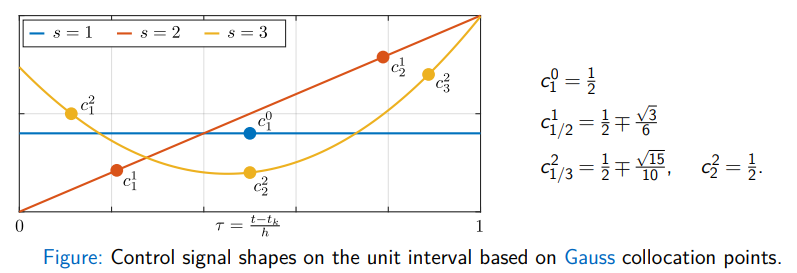
\includegraphics[width=0.8\linewidth]{pics/1656506685657.png}
		\label{fig:gausscoll}
	\end{figure}
\begin{itemize}
	\item Zero-order hold control input: $u(t) = {\color{red}{u_k^1}}$
	\item[~]
	\item First-order hold control input: $
		u(t) = {\color{red}{u_{k}^{1}}} l^{1}(t)+{\color{red}{u_{k}^{2}}} l^{2}(t)
		={\color{red}{u_{k}^{1}}} \frac{t-c_{2}^{1}}{c_{1}^{1}-c_{2}^{1}}+{\color{red}{u_{k}^{2}}} \frac{t-c_{1}^{1}}{c_{2}^{1}-c_{1}^{1}}$
\end{itemize}
\vspace{\baselineskip}
%RK coefficients:
%$$
%a_{i j}^{s} =\int_{0}^{c_{j}} \ell_{i}^{s-1}(\tau) d \tau, \quad b_{i}^{s} =\int_{0}^{1} \ell_{i}^{s-1}(\tau) d %\tau
%$$
\end{frame}

\begin{frame}
	\frametitle{Gauss collocation method}
	Numerical solution with {\color{red}{state stage values $x_k^i$}} and {\color{red}{control stage values $u_k^i$}}, $i = 1,...,s$:
	\\
	a) ZOH: 
	\begin{equation}
		\begin{split}
			x_{k+1}&=x_{k}+\Delta t  b_{1}  A_{\rm{con}}  {\color{red}{x_{k}^{1}}}+\Delta t  b_{1}  B_{\rm{con}}  {\color{red}{u_{k}^{1}}},\\
			{\color{red}{x_{k}^{1}}}&=x_{k}+\Delta t a_{11} A_{\rm{con}} {\color{red}{x_{k}^{1}}}+\Delta t  a_{11} B_{\rm{con}} {\color{red}{u_{k}^{1}}}.
		\end{split}
		\label{zerocoll}
	\end{equation}
    b) FOH:
    \begin{equation}
    	\begin{split}
    		x_{k+1}&=x_{k}+\Delta t  b_{1}  A_{\rm{con}}  {\color{red}{x_{k}^{1}}}+\Delta t  b_{2}  A_{\rm{con}}  {\color{red}{x_{k}^{2}}} \\ & \quad+\Delta t  b_{1}  B_{\rm{con}}  {\color{red}{u_{k}^{1}}}+\Delta t  b_{2}  B_{\rm{con}}  {\color{red}{u_{k}^{2}}}, \\
    		{\color{red}{x_{k}^{1}}}&=x_{k}+\Delta t  a_{11}  A_{\rm{con}}  {\color{red}{x_{k}^{1}}}+\Delta t  a_{12}  A_{\rm{con}}  {\color{red}{x_{k}^{2}}} \\ & \quad +\Delta t  a_{11}  B_{\rm{con}}  {\color{red}{u_{k}^{1}}}+\Delta t  a_{12}  B_{\rm{con}}  {\color{red}{u_{k}^{2}}}, \\
    		{\color{red}{x_{k}^{2}}}&=x_{k}+\Delta t  a_{21}  A_{\rm{con}}  {\color{red}{x_{k}^{1}}}+\Delta t  a_{22}  A_{\rm{con}}  {\color{red}{x_{k}^{2}}} \\ & \quad +\Delta t  a_{21}  B_{\rm{con}}  {\color{red}{u_{k}^{1}}}+\Delta t  a_{22}  B_{\rm{con}} {\color{red}{u_{k}^{2}}}.
    	\end{split}
    \end{equation}

\end{frame}

\section{Simulation and Results}

\begin{frame}
	\frametitle{Simulation setup}
	\begin{equation}
		\begin{split}
			A_{\text {con }}=\left[\begin{array}{cc}
				0 & 7.5 \\
				-1.5 & -0.1
			\end{array}\right], \quad B_{\text {con }}=\left[\begin{array}{c}
				0.145 \\
				0.5
			\end{array}\right].
		\end{split}
	\end{equation}
The initial condition is $x(0) = [2,2]^{\top}$ and the state and control input is subject to the following constraints
\begin{equation}
	\begin{split}
		-1 \leq\  &x_1 \leq 2.8\\
		-1 \leq\  &x_2 \leq 2.1\\
		-26 \leq\  &u \leq 26\\
	\end{split}
\end{equation}
\end{frame}

\begin{frame}
	\frametitle{Simulation setup}
The MPC solves the optimization problem:
$$
\min _{(x, u)} \sum_{k=i}^{i+N-1} l_{k}\left(x_{k}, u_{k}\right)+l_{N}\left(x_{k+N}\right),\forall k \in[i, \cdots, i+N-1]
$$
where
$$
\begin{aligned}
	l_{k} &=x_{k}^{T} Q x_{k}+u_{k}^{T} R u_{k}, \\
	l_{N} &=x_{k+N}^{T} Q_{N} x_{k+N}
\end{aligned}
$$
We set the prediction horizon $N = 10$, the weight matrices $Q =
Q_N =\text{diag}([10, 1])$ and $R = 1$.
\end{frame}

\begin{frame}
	\only<1>{
	\frametitle{Results of RK}
	\begin{figure}[H]
		\centering
		\begin{subfigure}[b]{0.49\textwidth}
			\centering
			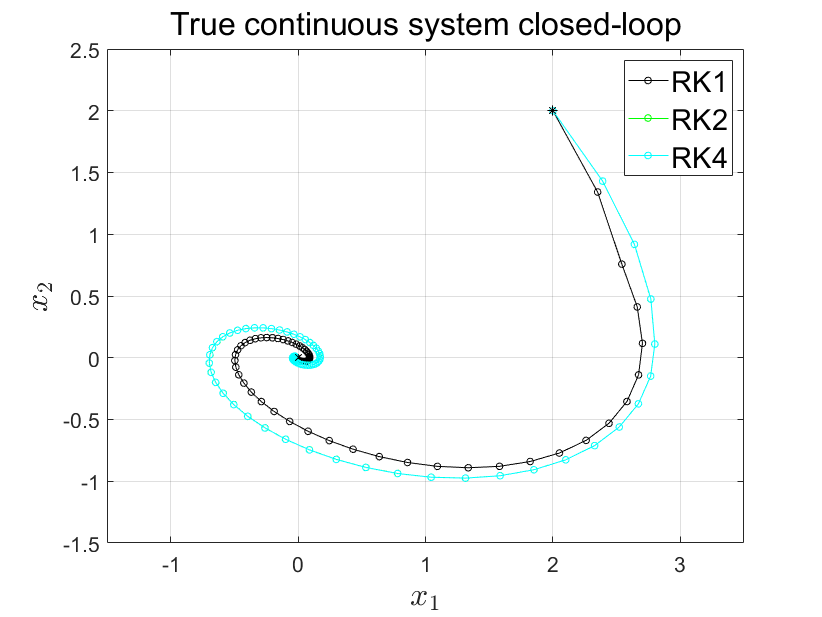
\includegraphics[width=\linewidth]{pics/deltat = 0.04.png}
			\caption{Sampling time $\Delta t = 0.04$ }
			\label{fig:statetrajec0.04}
		\end{subfigure}
		\hfill
		\begin{subfigure}[b]{0.49\textwidth}
			\centering
			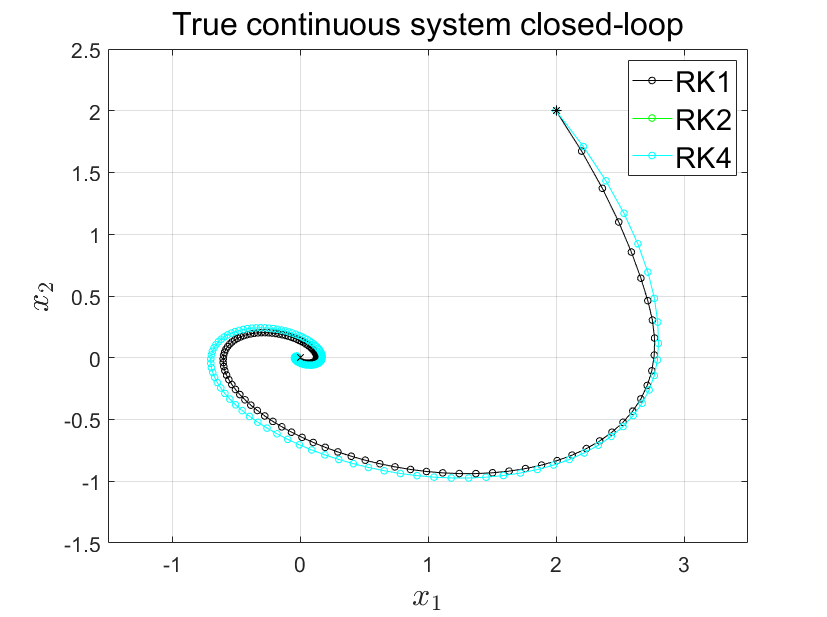
\includegraphics[width=\linewidth]{pics/deltat = 0.02.png}
			\caption{Sampling time $\Delta t = 0.02$}
			\label{fig:statetrajec0.02}
		\end{subfigure}
		%\caption{State trajectory of true continuous-time system}
		\label{State trajectory of true continuous system}
	\end{figure}}
%\end{frame}

%\begin{frame}
	\only<2>{
	\frametitle{Results of RK}
	\begin{figure}[h!]
		\centering
		\begin{subfigure}[h!]{0.49\textwidth}
			\centering
			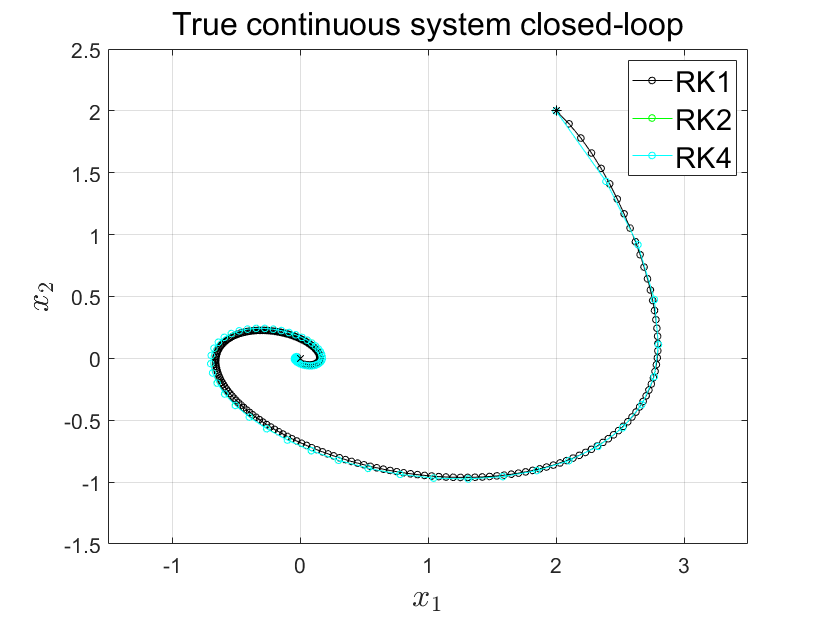
\includegraphics[width=\linewidth]{pics/delta0.04rk10.02rk2rk4.png}
			\caption{Sampling time $\Delta t\ = 0.008$ \text{for RK1}
				\\
			\quad \ \ Sampling time $\Delta t \ = 0.04$ \text{for RK2 and RK4}}
			\label{fig:statetrajec0.020.04}
		\end{subfigure}
		\hfill
		\begin{subfigure}[h!]{0.5\textwidth}
			\centering
			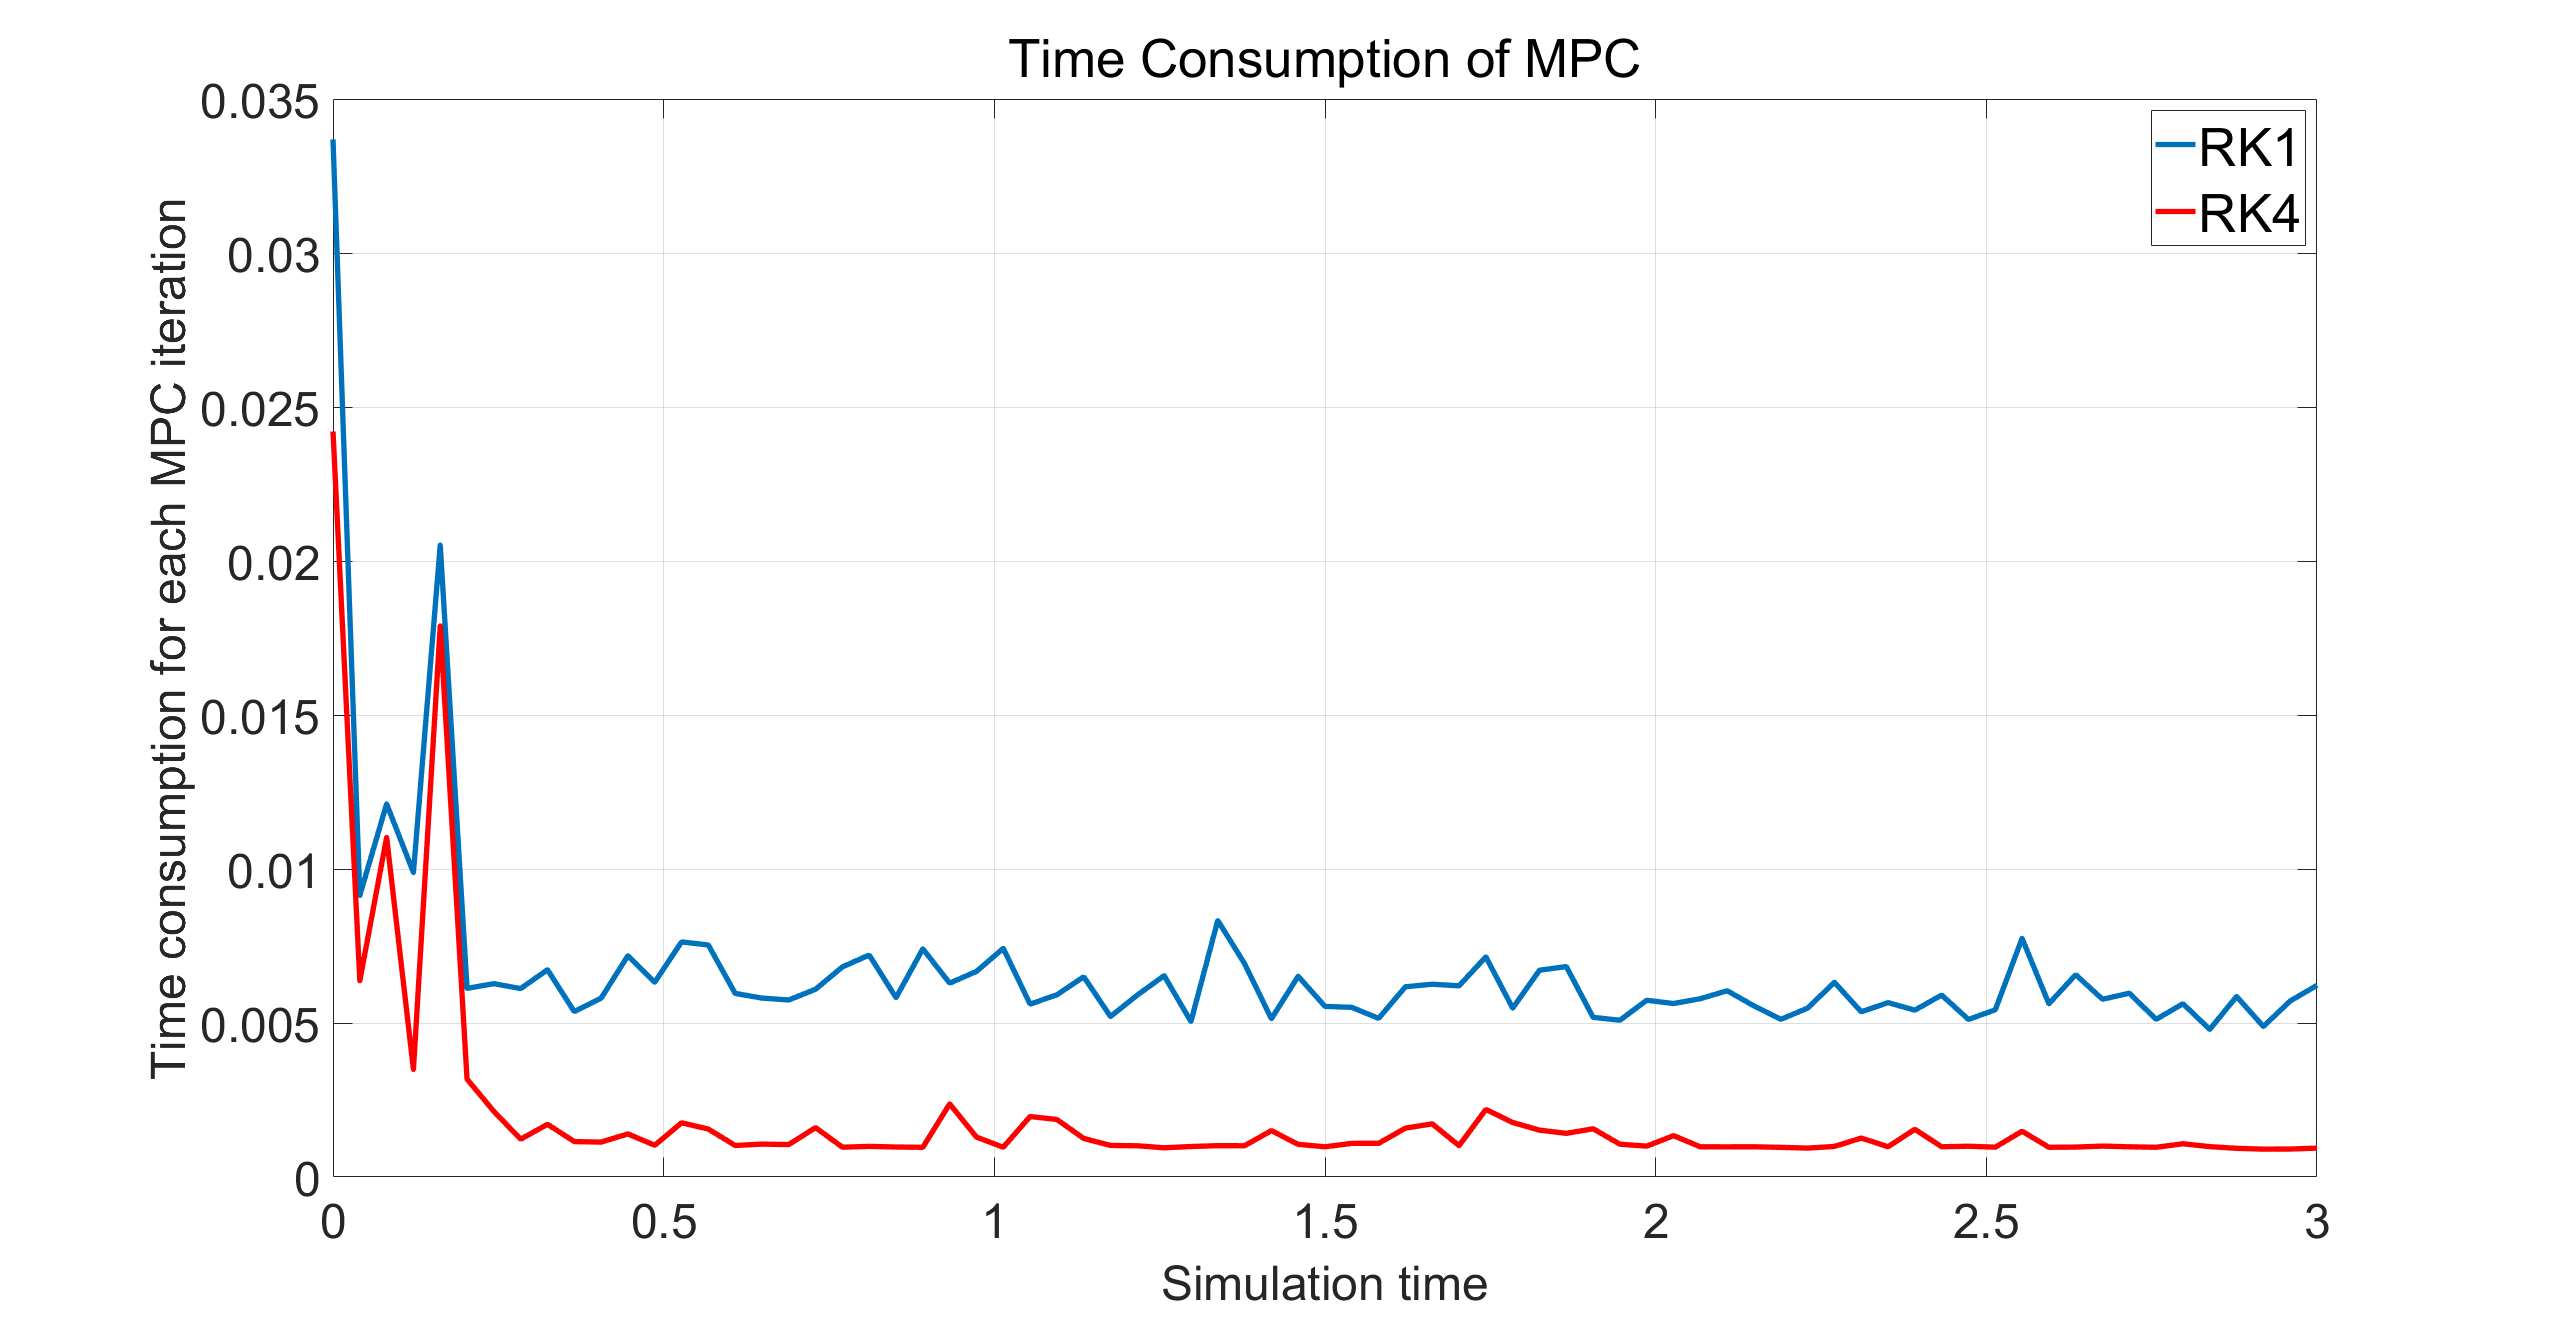
\includegraphics[width=\linewidth]{pics/timempc.png}
			\caption{Time consumption of MPC iteration}
			\label{fig:timempc}
		\end{subfigure}
		%\caption{?}
		\label{State trajectory of true continuous system}
	\end{figure}}
%\end{frame}

%\begin{frame}
	\only<3>{
	\frametitle{Results of RK}
	\begin{figure}[H]
		\centering
		\begin{subfigure}[b]{0.49\textwidth}
			\centering
			\includegraphics[width=\linewidth]{pics/coninvset0.06.png}
			\caption{The control invariant set for RK1 model \\ \quad \ \ in the case of $\Delta t = 0.06$}
			\label{fig:coninvesetrk1}
		\end{subfigure}
		\hfill
		\begin{subfigure}[b]{0.49\textwidth}
			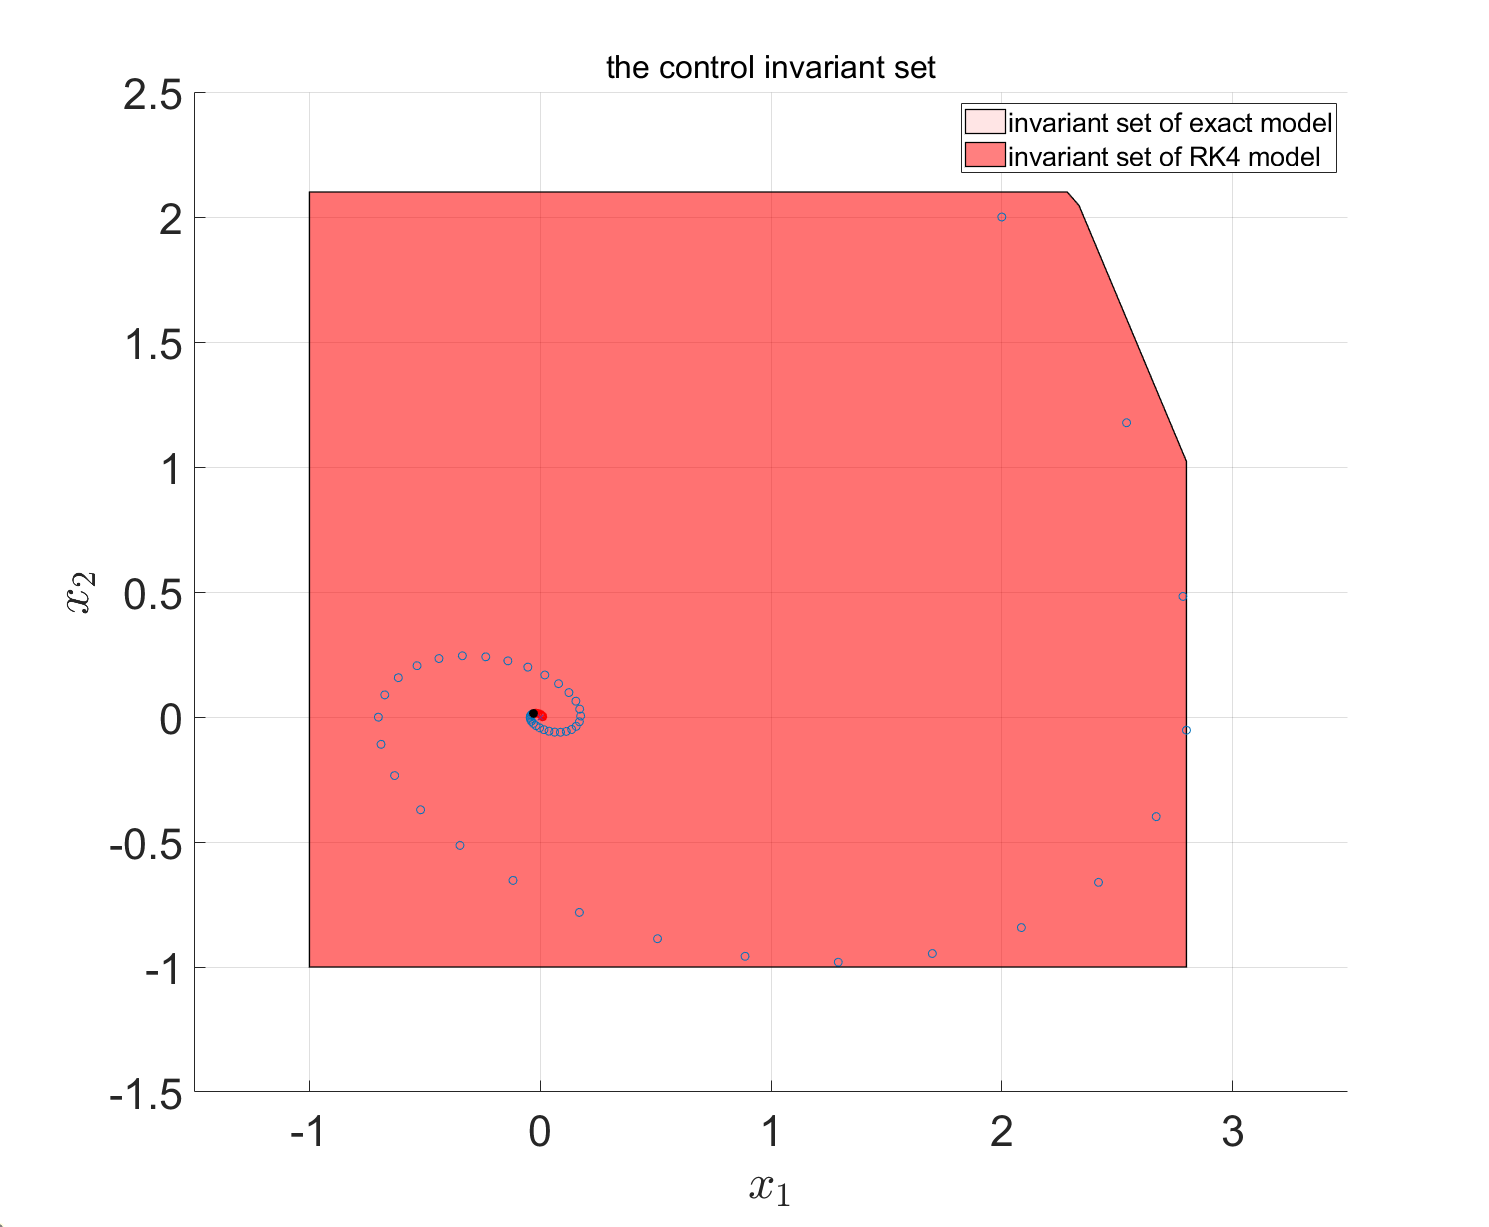
\includegraphics[width=\linewidth]{pics/CONINVSETRK40.06.png}
			\caption{The control invariant set for RK4 model \\ \quad \ \ in the case of $\Delta t = 0.06$}
			\label{fig:coninvesetrk4}
		\end{subfigure}
	%	\caption{The control invariant set}
		\label{The control invariant set}
	\end{figure}}
%\end{frame}

%\begin{frame}
	\only<4>{
	\frametitle{Results of RK}
	\begin{figure}[h!]
		\centering
		\begin{subfigure}[b]{0.49\textwidth}
			\centering
			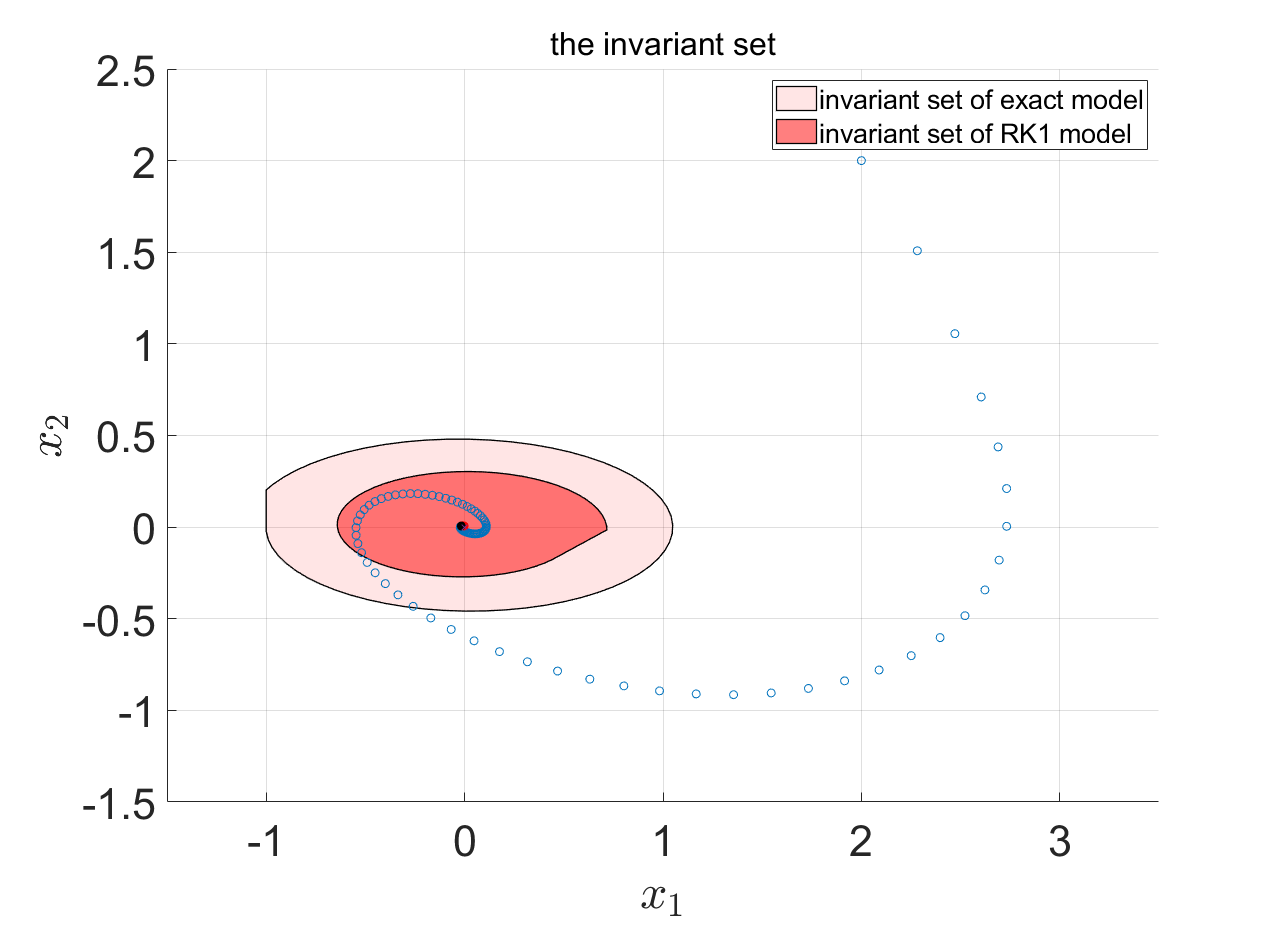
\includegraphics[width=\linewidth]{pics/invsetrk1.png}
			\caption{The invariant set of RK1 model \\ \quad \ \ in the case of $\Delta t = 0.06$}
			\label{fig:invesetrk1}
		\end{subfigure}
		\hfill
		\begin{subfigure}[b]{0.49\textwidth}
			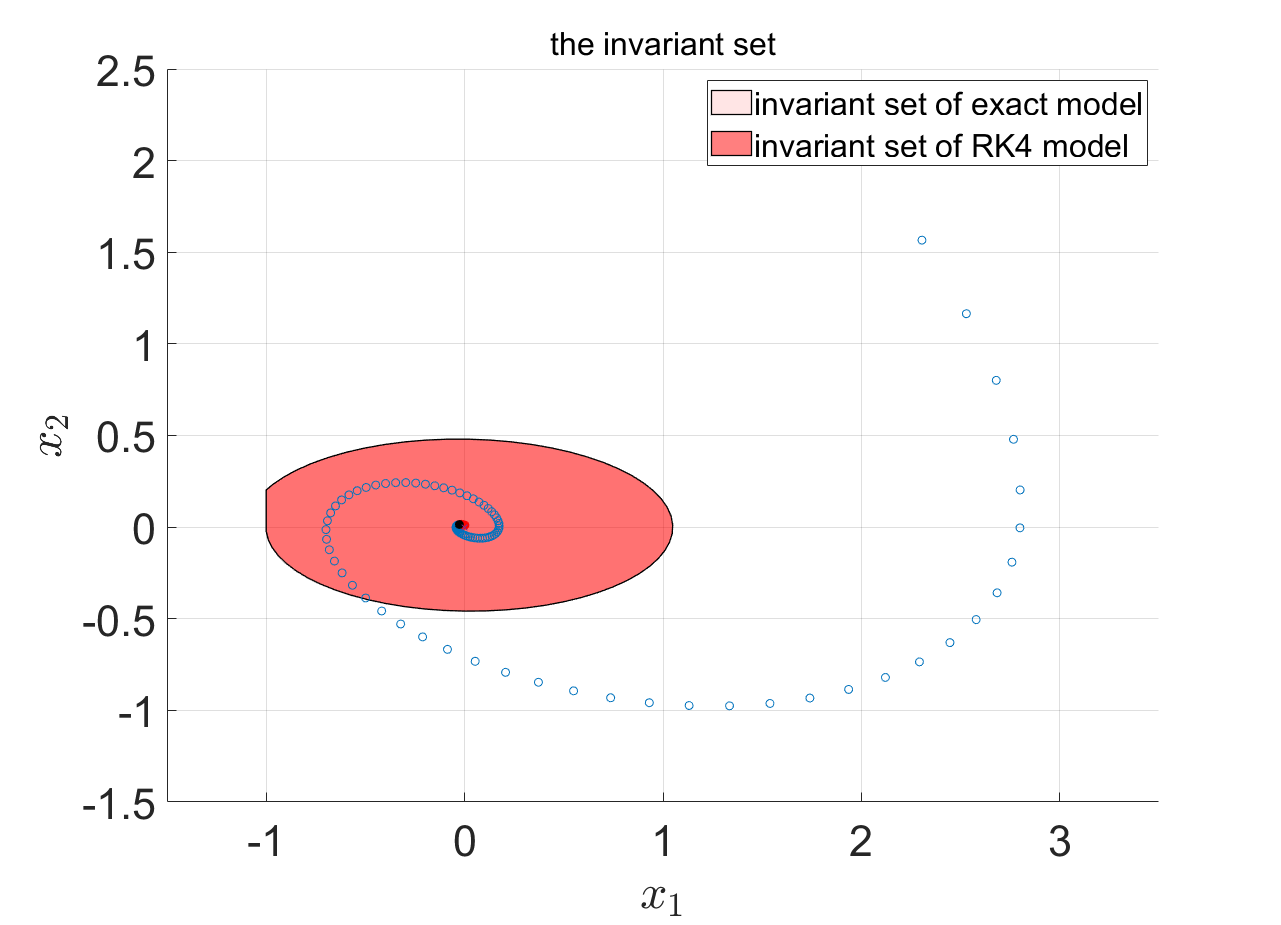
\includegraphics[width=\linewidth]{pics/invsetrk4.png}
			\caption{The invariant set of RK4 model \\ \quad \ \ in the case of $\Delta t = 0.06$}
			\label{fig:invesetrk4}
		\end{subfigure}
		%\caption{The invariant set}
		\label{fig:The invariant set}
	\end{figure}}
\end{frame}

\begin{frame}
	\only<1>{
	\frametitle{Results of Gauss collocation}
	\begin{figure}[H]
		\centering
		\begin{subfigure}[h!]{0.49\textwidth}
			\centering
			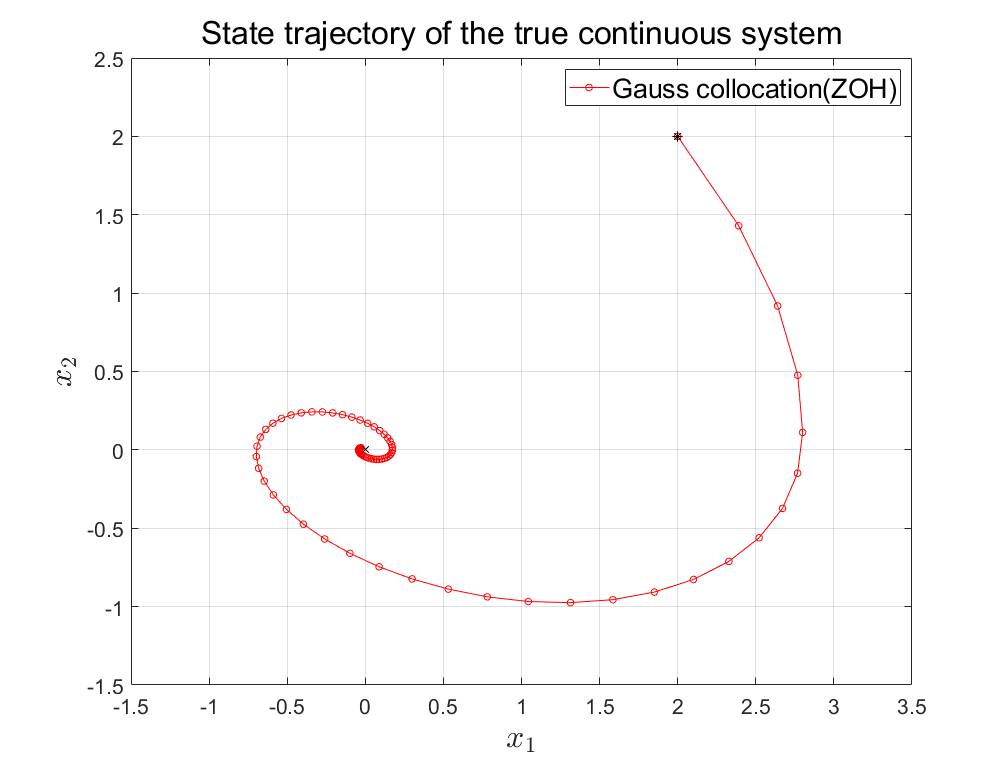
\includegraphics[width=\linewidth]{pics/gczero.png}
			\caption{State trajectory of the true continuous system for ZOH}
			\label{fig:gczero.png}
		\end{subfigure}
		\hfill
		\begin{subfigure}[h!]{0.5\textwidth}
			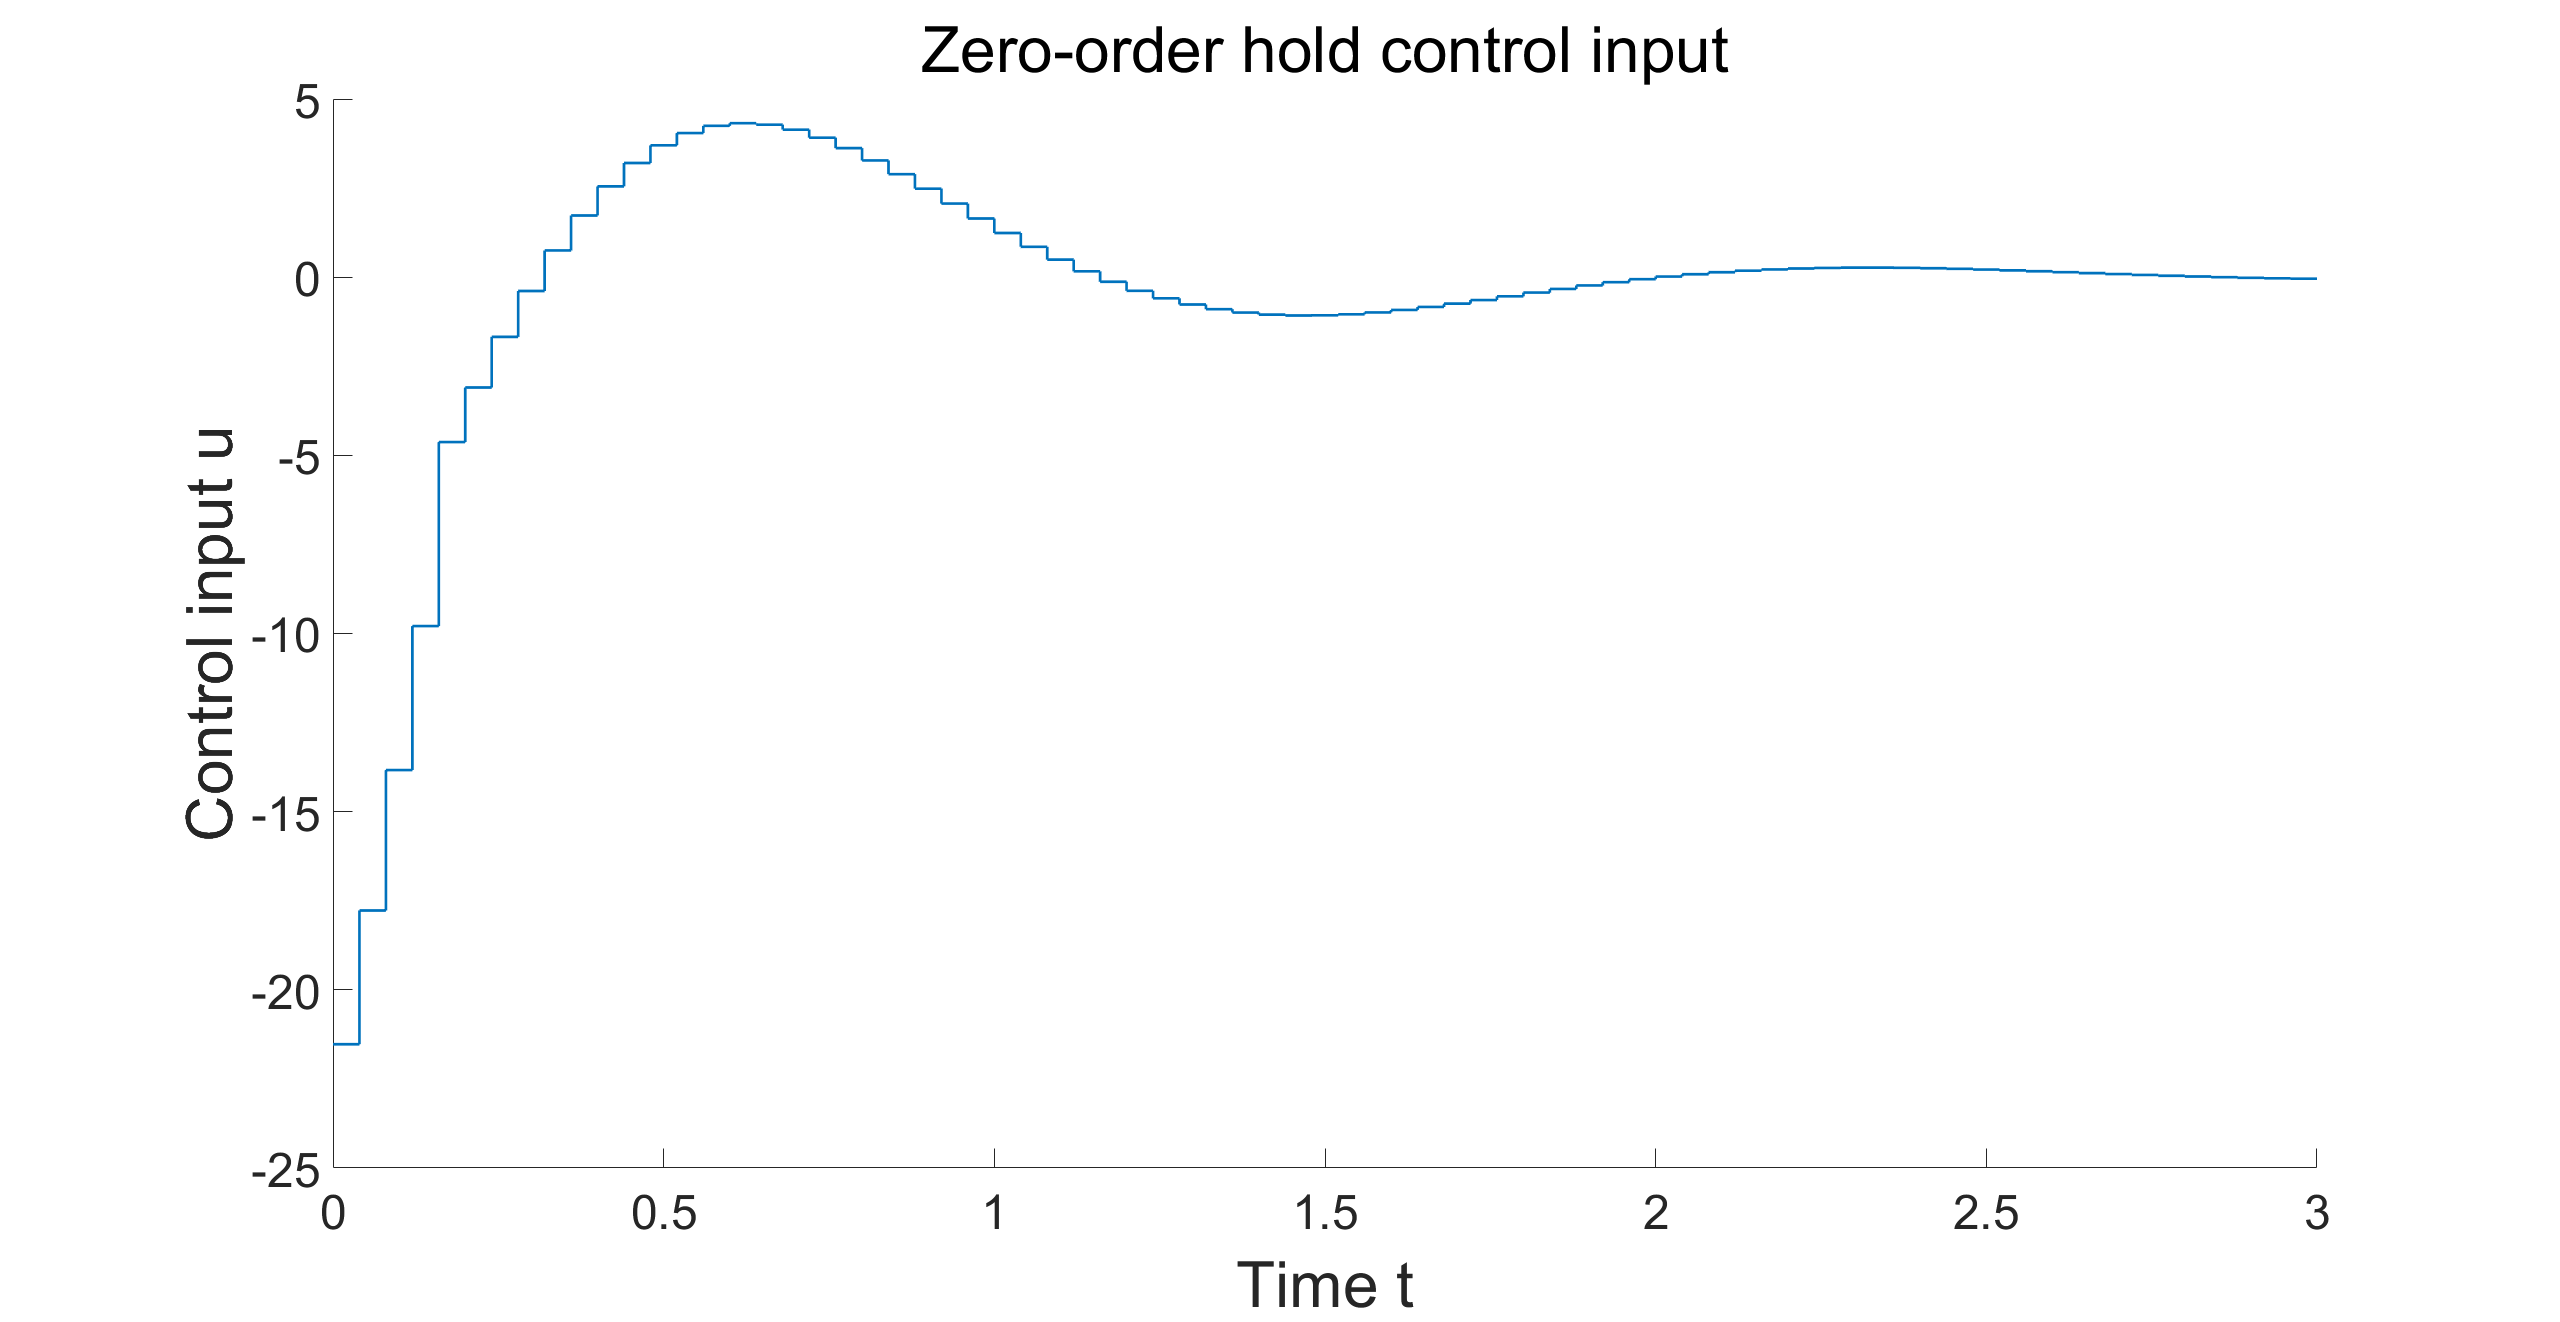
\includegraphics[width=\linewidth]{pics/ZOHINPUT.png}
			\caption{ZOH control input}
			\label{fig:ZOHINPUT}
		\end{subfigure}
		%\caption{The state trajectory and ZOH control input}
		\label{fig:The ZOH}
	\end{figure}}
%\end{frame}

%\begin{frame}
	\only<2>{
	\frametitle{Results of Gauss collocation}
	\begin{figure}[H]
		\centering
		\begin{subfigure}[h!]{0.49\textwidth}
			\centering
			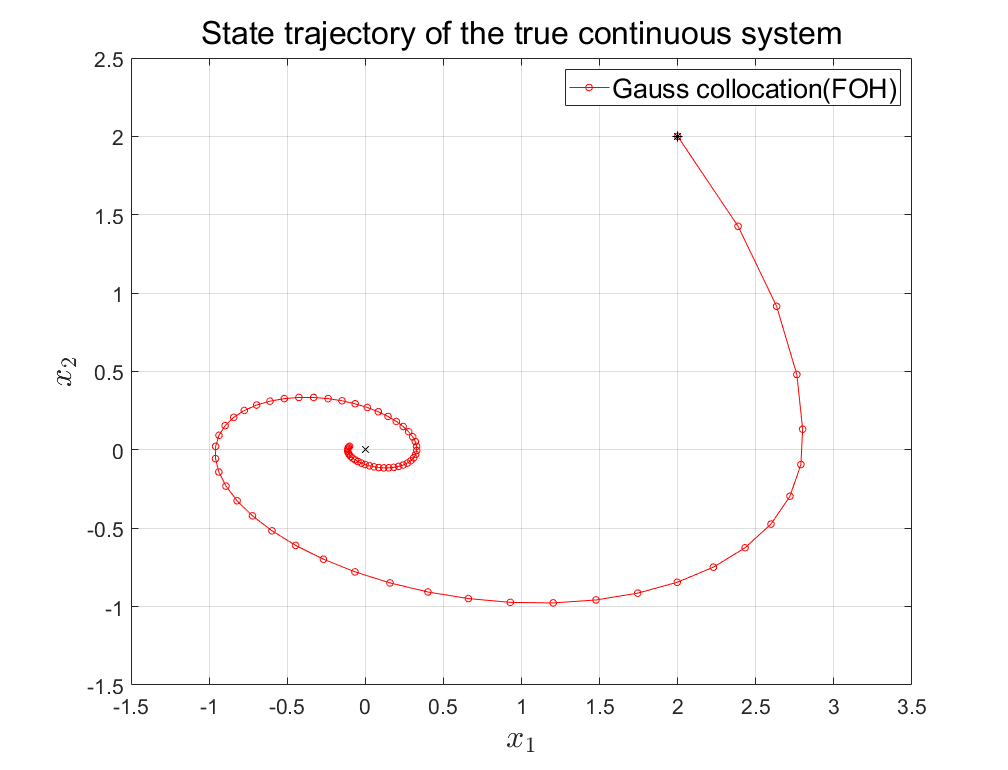
\includegraphics[width=\linewidth]{pics/gcfirst.png}
			\caption{State trajectory of the true continuous system for FOH}
			\label{fig:gcfirst.png}
		\end{subfigure}
		\hfill
		\begin{subfigure}[h!]{0.5\textwidth}
			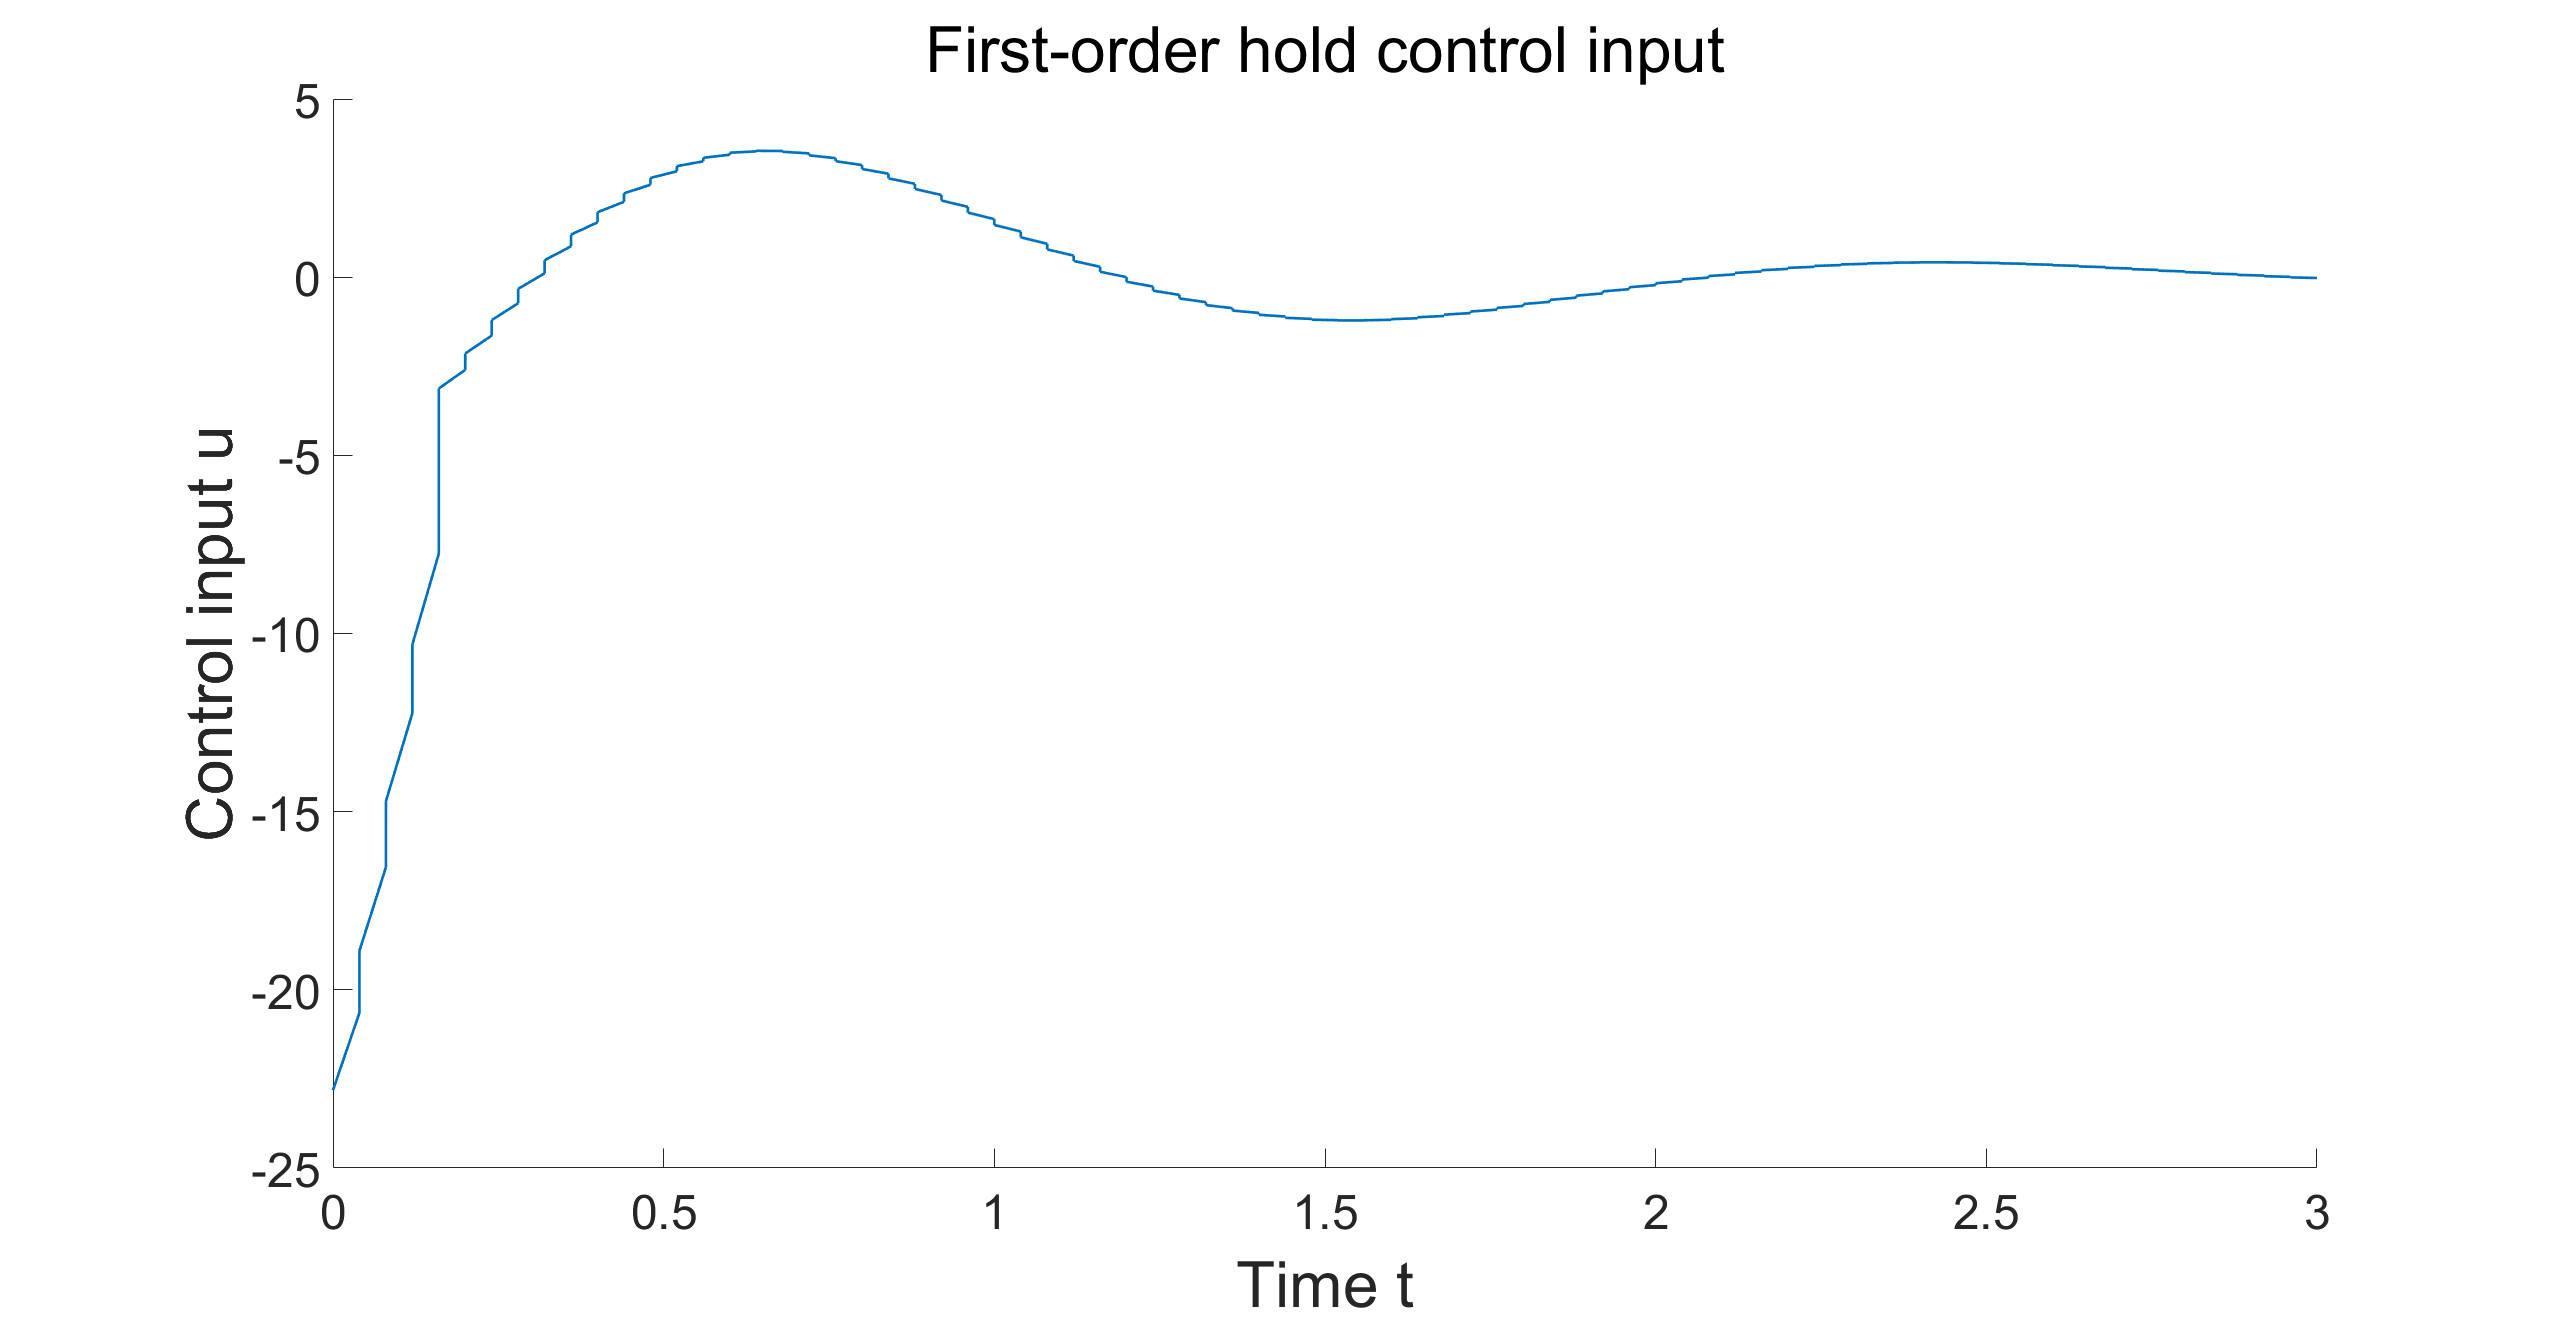
\includegraphics[width=\linewidth]{pics/FOHINPUT.png}
			\caption{FOH control input}
			\label{fig:FOHINPUT}
		\end{subfigure}
		%\caption{The state trajectory and ZOH control input}
		\label{fig:The FOH}
	\end{figure}}

    \only<3>{
    \frametitle{Results of Gauss collocation}
    \begin{figure}[H]
    	\centering
    	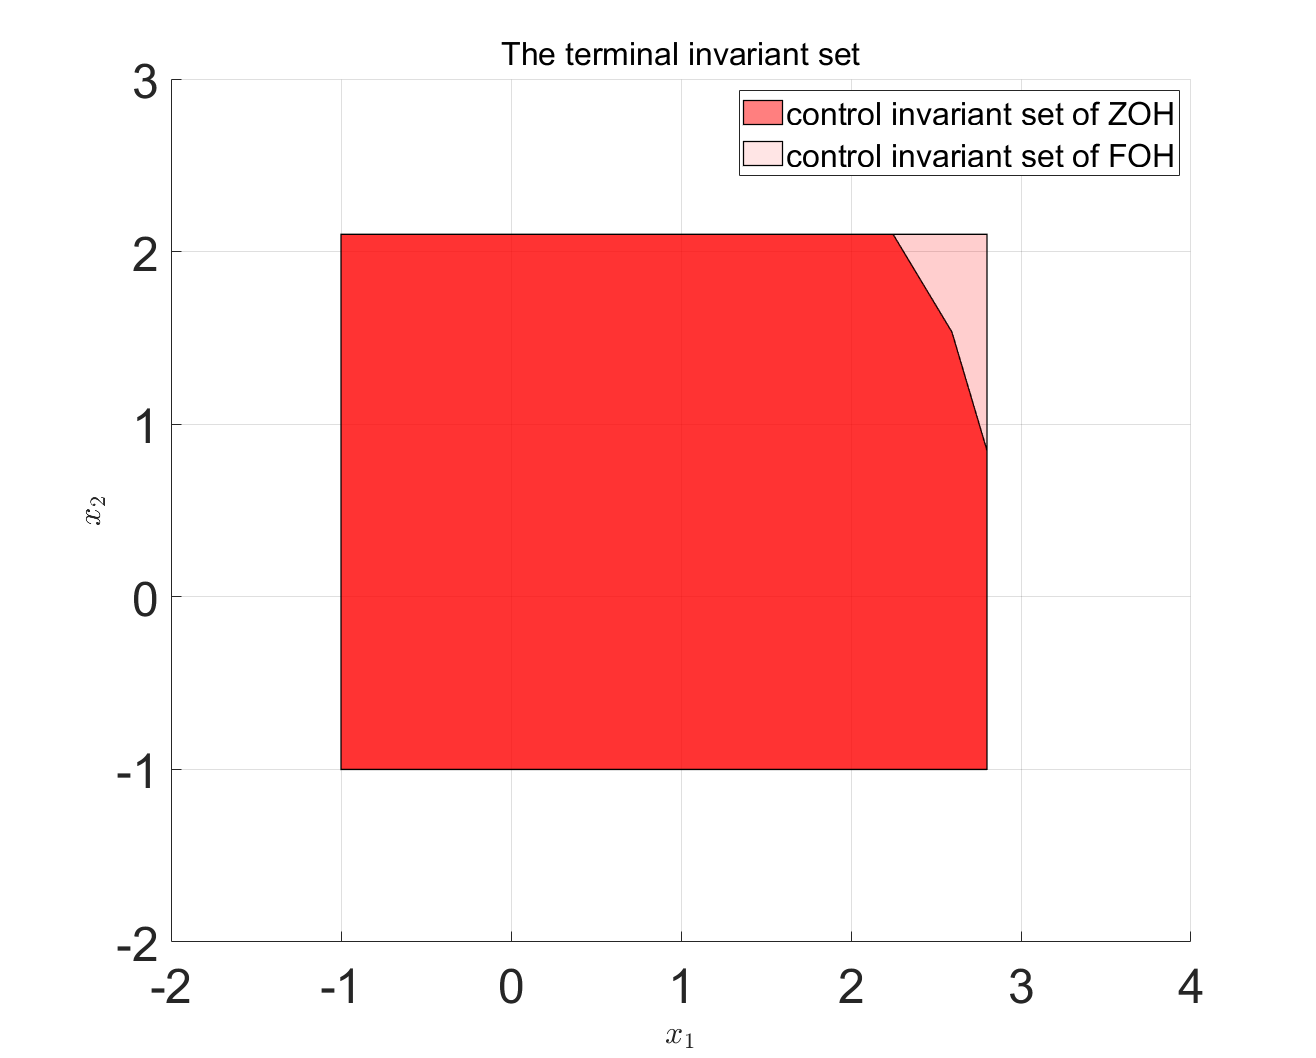
\includegraphics[width=0.5\linewidth]{pics/gcinvariantset.png}
    	\label{fig:gsconinvset}
    \end{figure}}
\end{frame}
%%%%%%%%%%%%%%%%%%%%%%%%%%%%%%%%%%%%%%%%%%%%%%%%%%%%%%%%%%%%%%%%%%%%%%%%%%%%%%%%%%%%%%%%%%%%%%%%%%%%%%%%%%%%%%%%%%%%%%%%%%%%%%%%%%%%%%%%%%%%%
% VIDEO: both examples below show a figure where the video will be displayed. 
% This figure could be a still picture of the video, giving a hint on what the video will show. 
% Usage of such a figure can be useful in case the presentation is likely to be printed as e.g. a handout 
% Please comment in slides shown below yourself for testing!
% NOTE: the folder containing the videos MUST BE INSIDE the presentation folder, otherwise the videos might not show up in the presentation.
% Also: the videos cannot be displayed on ubuntu, use e.g. the windows imperator to check whether the videos work

%video example1
% comment out manually
%{
%    \usebackgroundtemplate{\includemedia[width=12.8cm,height=9.6cm,activate=onclick,]{
\includegraphics{motivation}}{movie/example_video_short.swf}} 
%    \begin{frame}[plain]
%    \end{frame}
%}

%video example2
% \begin{frame}
% 	\frametitle{Example video}
% \includemedia[height=.5\textwidth]{
\includegraphics[height=.5\textwidth]{motivation}}{movie/example_video_short.swf} 
% \end{frame}
%%%%%%%%%%%%%%%%%%%%%%%%%%%%%%%%%%%%%%%%%%%%%%%%%%%%%%%%%%%%%%%%%%%%%%%%%%%%%%%%%%%%%%%%%%%%%%%%%%%%%%%%%%%%%%%%%%%%%%%%%%%%%%%%%%%%%%%%%%%%%%%%
\section{Conclusion}

\begin{frame}
	\frametitle{Conclusion}
	\begin{itemize}
		\item Increasing order of RK method $\rightarrow$ improved prediction accuracy \& closed-loop performance
		%The prediction accuracy and
		%closed-loop performance of MPC increased with increasing
		%order of the RK method
		\item[~]  
		\item RK1 with small $\Delta t$ $\approx$ RK4 with large $\Delta t$, but increased computational load.
		%we can achieve similar accuracy between RK1
		%with small sampling time and RK4 with large sampling time,
		%however, this yields increased computational cost due to the
		%increased number of optimization variables
		\item[~]
		\item Increased control invariant set for higher-order hold input
		%the control
		%invariant set of FOH control input is larger than ZOH control
		%input, as FOH can consider more input shapes than ZOH.
		\item[~]
	\end{itemize}
\begin{block}{Outlook:}
	\begin{itemize}
	    \item Nonlinear systems
	    \item Higher-order hold control inputs
	    \item Continuity constraint for control jumps
	\end{itemize}
\end{block}
	
\end{frame}

\appendix

%\begin{frame}[plain]
	% This slide serves 3 purposes:
	% 	1. a simple example how to create figures in tikz using beamer
	%	2. testing if you actually checked the content of this template
	% 	3. subtly preventing you from adding a "Thank you..." slide at the end of your presentation
	% If this slide is still in your final presentation... well, congratulation!
	%\begin{center}
	%	{\fontsize{40}{50} \structure{Sorry for your attention\\}}
	%	\renewcommand{\RobotName}{I}
	%	\resizebox {!} {0.16\textwidth} {\begin{tikzpicture}
	% nodes
	\begin{pgfonlayer}{nodelayer}
		\node (roboHead) {
			\begin{tikzpicture}
% nodes
\begin{pgfonlayer}{nodelayer}
	\node[robotRec](head){};
	\node[robotCirc, fill=white, minimum size=2pt, above=2pt of head.north](antennaBulb){};
	\node[robotCirc, fill=white, minimum size=7pt](eyeL)at ($(head.135)!0.4!(head.225)$){};
	\node[robotCirc, minimum size=1pt,scale=0.3](eyeLMid) at ($(head.135)!0.4!(head.225)$){};
	\node[robotCirc, fill=white, minimum size=7pt](eyeR) at ($(head.45) !0.4!(head.315)$){};
	\node[robotCirc, minimum size=1pt,scale=0.3](eyeRMid) at ($(head.45) !0.4!(head.315)$){};
\end{pgfonlayer}

% coordinate helpers
\coordinate (mouth1)  at ($(head.130)!0.73!(head.230)$);
\coordinate (mouth2)  at ($(head.50)!0.73!(head.310)$);
\coordinate (tongue)  at ($(mouth1)!0.88!(mouth2)$);

% edges (behind node layer)
\begin{pgfonlayer}{edgelayer}
	\draw[line width=3pt] (head.center) --  (antennaBulb.center) ;
\end{pgfonlayer}

% edges in foreground
\begin{pgfonlayer}{foreground}
	\draw[line width=2pt,line cap=round] (mouth1) --  (mouth2);
	\draw[line width=1.5pt] (tongue) arc[draw, start angle=0, end angle=-180, x radius=4pt, y radius=3pt];
\end{pgfonlayer}
\end{tikzpicture}
		};	
		\node[robotRec, minimum height=40pt, below=1pt of roboHead, anchor=north](body){\Large\RobotName};
		%feet
		\node[robotRec, minimum width=30pt, rounded corners=4pt, minimum height=10pt, below left = 2pt and -12pt of body, anchor=north](footL){};
		\node[robotRec, minimum width=30pt, rounded corners=4pt, minimum height=10pt, below right = 2pt and -12pt of body,anchor=north](footR){};
		\node[robotRec, minimum width=10pt, rounded corners=4pt, minimum height=30pt, below left = 2.5pt and -5pt of body.north west,anchor=north,rotate=-40](armL){};
		\node[robotRec, minimum width=10pt, rounded corners=4pt, minimum height=30pt, below right = 2pt and -1pt of body.north east,anchor=north](armR){};
	\end{pgfonlayer}
	
	% nodes in background 
	\begin{pgfonlayer}{background}	
		\node[robotRec, minimum width=15pt, rounded corners=2pt, minimum height=20pt, above=10pt of roboHead.south, anchor=north](neck){};
		\node[robotRec, minimum width=15pt, rounded corners=2pt, minimum height=20pt, above=10pt of footL.north, 	anchor=north](legL){};
		\node[robotRec, minimum width=15pt, rounded corners=2pt, minimum height=20pt, above=10pt of footR.north, anchor=north](legR){};
	\end{pgfonlayer}
	
	% coordinates
	\coordinate (handLCon)  at ($(armL.south)+(0pt,-9pt)$);
	\coordinate (handRCon)  at ($(armR.south)+(8pt,-8pt)$);
		
	% edges
	\begin{pgfonlayer}{foreground}
		\draw[line width=3pt,line cap=round] (handLCon) arc[draw, start angle=-40, end angle=145, x radius=8pt, y radius=8pt];
		\draw[line width=3pt,line cap=round] (handRCon) arc[draw, start angle=0, end angle=180, x radius=8pt, y radius=8pt];
	\end{pgfonlayer}
\end{tikzpicture}}
	%	\renewcommand{\RobotName}{DID}
	%	\resizebox {!} {0.16\textwidth} {\begin{tikzpicture}
	% nodes
	\begin{pgfonlayer}{nodelayer}
		\node (roboHead) {
			\begin{tikzpicture}
% nodes
\begin{pgfonlayer}{nodelayer}
	\node[robotRec](head){};
	\node[robotCirc, fill=white, minimum size=2pt, above=2pt of head.north](antennaBulb){};
	\node[robotCirc, fill=white, minimum size=7pt](eyeL)at ($(head.135)!0.4!(head.225)$){};
	\node[robotCirc, minimum size=1pt,scale=0.3](eyeLMid) at ($(head.135)!0.4!(head.225)$){};
	\node[robotCirc, fill=white, minimum size=7pt](eyeR) at ($(head.45) !0.4!(head.315)$){};
	\node[robotCirc, minimum size=1pt,scale=0.3](eyeRMid) at ($(head.45) !0.4!(head.315)$){};
\end{pgfonlayer}

% coordinate helpers
\coordinate (mouth1)  at ($(head.130)!0.73!(head.230)$);
\coordinate (mouth2)  at ($(head.50)!0.73!(head.310)$);
\coordinate (tongue)  at ($(mouth1)!0.88!(mouth2)$);

% edges (behind node layer)
\begin{pgfonlayer}{edgelayer}
	\draw[line width=3pt] (head.center) --  (antennaBulb.center) ;
\end{pgfonlayer}

% edges in foreground
\begin{pgfonlayer}{foreground}
	\draw[line width=2pt,line cap=round] (mouth1) --  (mouth2);
	\draw[line width=1.5pt] (tongue) arc[draw, start angle=0, end angle=-180, x radius=4pt, y radius=3pt];
\end{pgfonlayer}
\end{tikzpicture}
		};	
		\node[robotRec, minimum height=40pt, below=1pt of roboHead, anchor=north](body){\Large\RobotName};
		%feet
		\node[robotRec, minimum width=30pt, rounded corners=4pt, minimum height=10pt, below left = 2pt and -12pt of body, anchor=north](footL){};
		\node[robotRec, minimum width=30pt, rounded corners=4pt, minimum height=10pt, below right = 2pt and -12pt of body,anchor=north](footR){};
		\node[robotRec, minimum width=10pt, rounded corners=4pt, minimum height=30pt, below left = 2.5pt and -5pt of body.north west,anchor=north,rotate=-40](armL){};
		\node[robotRec, minimum width=10pt, rounded corners=4pt, minimum height=30pt, below right = 2pt and -1pt of body.north east,anchor=north](armR){};
	\end{pgfonlayer}
	
	% nodes in background 
	\begin{pgfonlayer}{background}	
		\node[robotRec, minimum width=15pt, rounded corners=2pt, minimum height=20pt, above=10pt of roboHead.south, anchor=north](neck){};
		\node[robotRec, minimum width=15pt, rounded corners=2pt, minimum height=20pt, above=10pt of footL.north, 	anchor=north](legL){};
		\node[robotRec, minimum width=15pt, rounded corners=2pt, minimum height=20pt, above=10pt of footR.north, anchor=north](legR){};
	\end{pgfonlayer}
	
	% coordinates
	\coordinate (handLCon)  at ($(armL.south)+(0pt,-9pt)$);
	\coordinate (handRCon)  at ($(armR.south)+(8pt,-8pt)$);
		
	% edges
	\begin{pgfonlayer}{foreground}
		\draw[line width=3pt,line cap=round] (handLCon) arc[draw, start angle=-40, end angle=145, x radius=8pt, y radius=8pt];
		\draw[line width=3pt,line cap=round] (handRCon) arc[draw, start angle=0, end angle=180, x radius=8pt, y radius=8pt];
	\end{pgfonlayer}
\end{tikzpicture}}
	%	\renewcommand{\RobotName}{NOT}
	%	\resizebox {!} {0.16\textwidth} {\begin{tikzpicture}
	% nodes
	\begin{pgfonlayer}{nodelayer}
		\node (roboHead) {
			\begin{tikzpicture}
% nodes
\begin{pgfonlayer}{nodelayer}
	\node[robotRec](head){};
	\node[robotCirc, fill=white, minimum size=2pt, above=2pt of head.north](antennaBulb){};
	\node[robotCirc, fill=white, minimum size=7pt](eyeL)at ($(head.135)!0.4!(head.225)$){};
	\node[robotCirc, minimum size=1pt,scale=0.3](eyeLMid) at ($(head.135)!0.4!(head.225)$){};
	\node[robotCirc, fill=white, minimum size=7pt](eyeR) at ($(head.45) !0.4!(head.315)$){};
	\node[robotCirc, minimum size=1pt,scale=0.3](eyeRMid) at ($(head.45) !0.4!(head.315)$){};
\end{pgfonlayer}

% coordinate helpers
\coordinate (mouth1)  at ($(head.130)!0.73!(head.230)$);
\coordinate (mouth2)  at ($(head.50)!0.73!(head.310)$);
\coordinate (tongue)  at ($(mouth1)!0.88!(mouth2)$);

% edges (behind node layer)
\begin{pgfonlayer}{edgelayer}
	\draw[line width=3pt] (head.center) --  (antennaBulb.center) ;
\end{pgfonlayer}

% edges in foreground
\begin{pgfonlayer}{foreground}
	\draw[line width=2pt,line cap=round] (mouth1) --  (mouth2);
	\draw[line width=1.5pt] (tongue) arc[draw, start angle=0, end angle=-180, x radius=4pt, y radius=3pt];
\end{pgfonlayer}
\end{tikzpicture}
		};	
		\node[robotRec, minimum height=40pt, below=1pt of roboHead, anchor=north](body){\Large\RobotName};
		%feet
		\node[robotRec, minimum width=30pt, rounded corners=4pt, minimum height=10pt, below left = 2pt and -12pt of body, anchor=north](footL){};
		\node[robotRec, minimum width=30pt, rounded corners=4pt, minimum height=10pt, below right = 2pt and -12pt of body,anchor=north](footR){};
		\node[robotRec, minimum width=10pt, rounded corners=4pt, minimum height=30pt, below left = 2.5pt and -5pt of body.north west,anchor=north,rotate=-40](armL){};
		\node[robotRec, minimum width=10pt, rounded corners=4pt, minimum height=30pt, below right = 2pt and -1pt of body.north east,anchor=north](armR){};
	\end{pgfonlayer}
	
	% nodes in background 
	\begin{pgfonlayer}{background}	
		\node[robotRec, minimum width=15pt, rounded corners=2pt, minimum height=20pt, above=10pt of roboHead.south, anchor=north](neck){};
		\node[robotRec, minimum width=15pt, rounded corners=2pt, minimum height=20pt, above=10pt of footL.north, 	anchor=north](legL){};
		\node[robotRec, minimum width=15pt, rounded corners=2pt, minimum height=20pt, above=10pt of footR.north, anchor=north](legR){};
	\end{pgfonlayer}
	
	% coordinates
	\coordinate (handLCon)  at ($(armL.south)+(0pt,-9pt)$);
	\coordinate (handRCon)  at ($(armR.south)+(8pt,-8pt)$);
		
	% edges
	\begin{pgfonlayer}{foreground}
		\draw[line width=3pt,line cap=round] (handLCon) arc[draw, start angle=-40, end angle=145, x radius=8pt, y radius=8pt];
		\draw[line width=3pt,line cap=round] (handRCon) arc[draw, start angle=0, end angle=180, x radius=8pt, y radius=8pt];
	\end{pgfonlayer}
\end{tikzpicture}}
	%	\renewcommand{\RobotName}{CHECK}
	%	\resizebox {!} {0.16\textwidth} {\begin{tikzpicture}
	% nodes
	\begin{pgfonlayer}{nodelayer}
		\node (roboHead) {
			\begin{tikzpicture}
% nodes
\begin{pgfonlayer}{nodelayer}
	\node[robotRec](head){};
	\node[robotCirc, fill=white, minimum size=2pt, above=2pt of head.north](antennaBulb){};
	\node[robotCirc, fill=white, minimum size=7pt](eyeL)at ($(head.135)!0.4!(head.225)$){};
	\node[robotCirc, minimum size=1pt,scale=0.3](eyeLMid) at ($(head.135)!0.4!(head.225)$){};
	\node[robotCirc, fill=white, minimum size=7pt](eyeR) at ($(head.45) !0.4!(head.315)$){};
	\node[robotCirc, minimum size=1pt,scale=0.3](eyeRMid) at ($(head.45) !0.4!(head.315)$){};
\end{pgfonlayer}

% coordinate helpers
\coordinate (mouth1)  at ($(head.130)!0.73!(head.230)$);
\coordinate (mouth2)  at ($(head.50)!0.73!(head.310)$);
\coordinate (tongue)  at ($(mouth1)!0.88!(mouth2)$);

% edges (behind node layer)
\begin{pgfonlayer}{edgelayer}
	\draw[line width=3pt] (head.center) --  (antennaBulb.center) ;
\end{pgfonlayer}

% edges in foreground
\begin{pgfonlayer}{foreground}
	\draw[line width=2pt,line cap=round] (mouth1) --  (mouth2);
	\draw[line width=1.5pt] (tongue) arc[draw, start angle=0, end angle=-180, x radius=4pt, y radius=3pt];
\end{pgfonlayer}
\end{tikzpicture}
		};	
		\node[robotRec, minimum height=40pt, below=1pt of roboHead, anchor=north](body){\Large\RobotName};
		%feet
		\node[robotRec, minimum width=30pt, rounded corners=4pt, minimum height=10pt, below left = 2pt and -12pt of body, anchor=north](footL){};
		\node[robotRec, minimum width=30pt, rounded corners=4pt, minimum height=10pt, below right = 2pt and -12pt of body,anchor=north](footR){};
		\node[robotRec, minimum width=10pt, rounded corners=4pt, minimum height=30pt, below left = 2.5pt and -5pt of body.north west,anchor=north,rotate=-40](armL){};
		\node[robotRec, minimum width=10pt, rounded corners=4pt, minimum height=30pt, below right = 2pt and -1pt of body.north east,anchor=north](armR){};
	\end{pgfonlayer}
	
	% nodes in background 
	\begin{pgfonlayer}{background}	
		\node[robotRec, minimum width=15pt, rounded corners=2pt, minimum height=20pt, above=10pt of roboHead.south, anchor=north](neck){};
		\node[robotRec, minimum width=15pt, rounded corners=2pt, minimum height=20pt, above=10pt of footL.north, 	anchor=north](legL){};
		\node[robotRec, minimum width=15pt, rounded corners=2pt, minimum height=20pt, above=10pt of footR.north, anchor=north](legR){};
	\end{pgfonlayer}
	
	% coordinates
	\coordinate (handLCon)  at ($(armL.south)+(0pt,-9pt)$);
	\coordinate (handRCon)  at ($(armR.south)+(8pt,-8pt)$);
		
	% edges
	\begin{pgfonlayer}{foreground}
		\draw[line width=3pt,line cap=round] (handLCon) arc[draw, start angle=-40, end angle=145, x radius=8pt, y radius=8pt];
		\draw[line width=3pt,line cap=round] (handRCon) arc[draw, start angle=0, end angle=180, x radius=8pt, y radius=8pt];
	\end{pgfonlayer}
\end{tikzpicture}}
	%	\renewcommand{\RobotName}{THIS}
	%	\resizebox {!} {0.16\textwidth} {\begin{tikzpicture}
	% nodes
	\begin{pgfonlayer}{nodelayer}
		\node (roboHead) {
			\begin{tikzpicture}
% nodes
\begin{pgfonlayer}{nodelayer}
	\node[robotRec](head){};
	\node[robotCirc, fill=white, minimum size=2pt, above=2pt of head.north](antennaBulb){};
	\node[robotCirc, fill=white, minimum size=7pt](eyeL)at ($(head.135)!0.4!(head.225)$){};
	\node[robotCirc, minimum size=1pt,scale=0.3](eyeLMid) at ($(head.135)!0.4!(head.225)$){};
	\node[robotCirc, fill=white, minimum size=7pt](eyeR) at ($(head.45) !0.4!(head.315)$){};
	\node[robotCirc, minimum size=1pt,scale=0.3](eyeRMid) at ($(head.45) !0.4!(head.315)$){};
\end{pgfonlayer}

% coordinate helpers
\coordinate (mouth1)  at ($(head.130)!0.73!(head.230)$);
\coordinate (mouth2)  at ($(head.50)!0.73!(head.310)$);
\coordinate (tongue)  at ($(mouth1)!0.88!(mouth2)$);

% edges (behind node layer)
\begin{pgfonlayer}{edgelayer}
	\draw[line width=3pt] (head.center) --  (antennaBulb.center) ;
\end{pgfonlayer}

% edges in foreground
\begin{pgfonlayer}{foreground}
	\draw[line width=2pt,line cap=round] (mouth1) --  (mouth2);
	\draw[line width=1.5pt] (tongue) arc[draw, start angle=0, end angle=-180, x radius=4pt, y radius=3pt];
\end{pgfonlayer}
\end{tikzpicture}
		};	
		\node[robotRec, minimum height=40pt, below=1pt of roboHead, anchor=north](body){\Large\RobotName};
		%feet
		\node[robotRec, minimum width=30pt, rounded corners=4pt, minimum height=10pt, below left = 2pt and -12pt of body, anchor=north](footL){};
		\node[robotRec, minimum width=30pt, rounded corners=4pt, minimum height=10pt, below right = 2pt and -12pt of body,anchor=north](footR){};
		\node[robotRec, minimum width=10pt, rounded corners=4pt, minimum height=30pt, below left = 2.5pt and -5pt of body.north west,anchor=north,rotate=-40](armL){};
		\node[robotRec, minimum width=10pt, rounded corners=4pt, minimum height=30pt, below right = 2pt and -1pt of body.north east,anchor=north](armR){};
	\end{pgfonlayer}
	
	% nodes in background 
	\begin{pgfonlayer}{background}	
		\node[robotRec, minimum width=15pt, rounded corners=2pt, minimum height=20pt, above=10pt of roboHead.south, anchor=north](neck){};
		\node[robotRec, minimum width=15pt, rounded corners=2pt, minimum height=20pt, above=10pt of footL.north, 	anchor=north](legL){};
		\node[robotRec, minimum width=15pt, rounded corners=2pt, minimum height=20pt, above=10pt of footR.north, anchor=north](legR){};
	\end{pgfonlayer}
	
	% coordinates
	\coordinate (handLCon)  at ($(armL.south)+(0pt,-9pt)$);
	\coordinate (handRCon)  at ($(armR.south)+(8pt,-8pt)$);
		
	% edges
	\begin{pgfonlayer}{foreground}
		\draw[line width=3pt,line cap=round] (handLCon) arc[draw, start angle=-40, end angle=145, x radius=8pt, y radius=8pt];
		\draw[line width=3pt,line cap=round] (handRCon) arc[draw, start angle=0, end angle=180, x radius=8pt, y radius=8pt];
	\end{pgfonlayer}
\end{tikzpicture}}
	%	\renewcommand{\RobotName}{SLIDE}
	%	\resizebox {!} {0.16\textwidth} {\begin{tikzpicture}
	% nodes
	\begin{pgfonlayer}{nodelayer}
		\node (roboHead) {
			\begin{tikzpicture}
% nodes
\begin{pgfonlayer}{nodelayer}
	\node[robotRec](head){};
	\node[robotCirc, fill=white, minimum size=2pt, above=2pt of head.north](antennaBulb){};
	\node[robotCirc, fill=white, minimum size=7pt](eyeL)at ($(head.135)!0.4!(head.225)$){};
	\node[robotCirc, minimum size=1pt,scale=0.3](eyeLMid) at ($(head.135)!0.4!(head.225)$){};
	\node[robotCirc, fill=white, minimum size=7pt](eyeR) at ($(head.45) !0.4!(head.315)$){};
	\node[robotCirc, minimum size=1pt,scale=0.3](eyeRMid) at ($(head.45) !0.4!(head.315)$){};
\end{pgfonlayer}

% coordinate helpers
\coordinate (mouth1)  at ($(head.130)!0.73!(head.230)$);
\coordinate (mouth2)  at ($(head.50)!0.73!(head.310)$);
\coordinate (tongue)  at ($(mouth1)!0.88!(mouth2)$);

% edges (behind node layer)
\begin{pgfonlayer}{edgelayer}
	\draw[line width=3pt] (head.center) --  (antennaBulb.center) ;
\end{pgfonlayer}

% edges in foreground
\begin{pgfonlayer}{foreground}
	\draw[line width=2pt,line cap=round] (mouth1) --  (mouth2);
	\draw[line width=1.5pt] (tongue) arc[draw, start angle=0, end angle=-180, x radius=4pt, y radius=3pt];
\end{pgfonlayer}
\end{tikzpicture}
		};	
		\node[robotRec, minimum height=40pt, below=1pt of roboHead, anchor=north](body){\Large\RobotName};
		%feet
		\node[robotRec, minimum width=30pt, rounded corners=4pt, minimum height=10pt, below left = 2pt and -12pt of body, anchor=north](footL){};
		\node[robotRec, minimum width=30pt, rounded corners=4pt, minimum height=10pt, below right = 2pt and -12pt of body,anchor=north](footR){};
		\node[robotRec, minimum width=10pt, rounded corners=4pt, minimum height=30pt, below left = 2.5pt and -5pt of body.north west,anchor=north,rotate=-40](armL){};
		\node[robotRec, minimum width=10pt, rounded corners=4pt, minimum height=30pt, below right = 2pt and -1pt of body.north east,anchor=north](armR){};
	\end{pgfonlayer}
	
	% nodes in background 
	\begin{pgfonlayer}{background}	
		\node[robotRec, minimum width=15pt, rounded corners=2pt, minimum height=20pt, above=10pt of roboHead.south, anchor=north](neck){};
		\node[robotRec, minimum width=15pt, rounded corners=2pt, minimum height=20pt, above=10pt of footL.north, 	anchor=north](legL){};
		\node[robotRec, minimum width=15pt, rounded corners=2pt, minimum height=20pt, above=10pt of footR.north, anchor=north](legR){};
	\end{pgfonlayer}
	
	% coordinates
	\coordinate (handLCon)  at ($(armL.south)+(0pt,-9pt)$);
	\coordinate (handRCon)  at ($(armR.south)+(8pt,-8pt)$);
		
	% edges
	\begin{pgfonlayer}{foreground}
		\draw[line width=3pt,line cap=round] (handLCon) arc[draw, start angle=-40, end angle=145, x radius=8pt, y radius=8pt];
		\draw[line width=3pt,line cap=round] (handRCon) arc[draw, start angle=0, end angle=180, x radius=8pt, y radius=8pt];
	\end{pgfonlayer}
\end{tikzpicture}}
	%	\hfill %
%	\end{center}
%\end{frame}


%\nocite{buss11}
%\nocite{bauer09}
\begin{frame}{\LSRITRRefTitle}
	\printbibliography	
\end{frame}


\end{document}
